%! TeX program = lualatex
\documentclass[main]{subfiles}

\begin{document}

\title[AutoML: BO]{Posterior Uncertainty and Acquisition Functions II}
\subtitle{Probability of Improvement and Expected Improvement}
\author[Bernd Bischl]{Bernd Bischl}
\date{}

\titlebackground*{images/AutoML_HPO_2_2}

%\institute{}
%\date{}

    \maketitle


\begin{frame}{Probability of Improvement}
    \textbf{Goal:} Find $\xvsi[t+1]$ that maximizes the \textbf{Probability of Improvement} (PI):
    $$a_{\text{PI}}(\xv) = \P(Y(\xv) < \fmin) = \Phi\!\left(\frac{\fmin - \surro(\xv)}{\sh(\xv)}\right)$$
    where $\Phi(\cdot)$ is the standard normal cdf (assuming Gaussian posterior).
    \vfill
    \begin{columns}
        \column{.5\textwidth}
        \begin{center}
            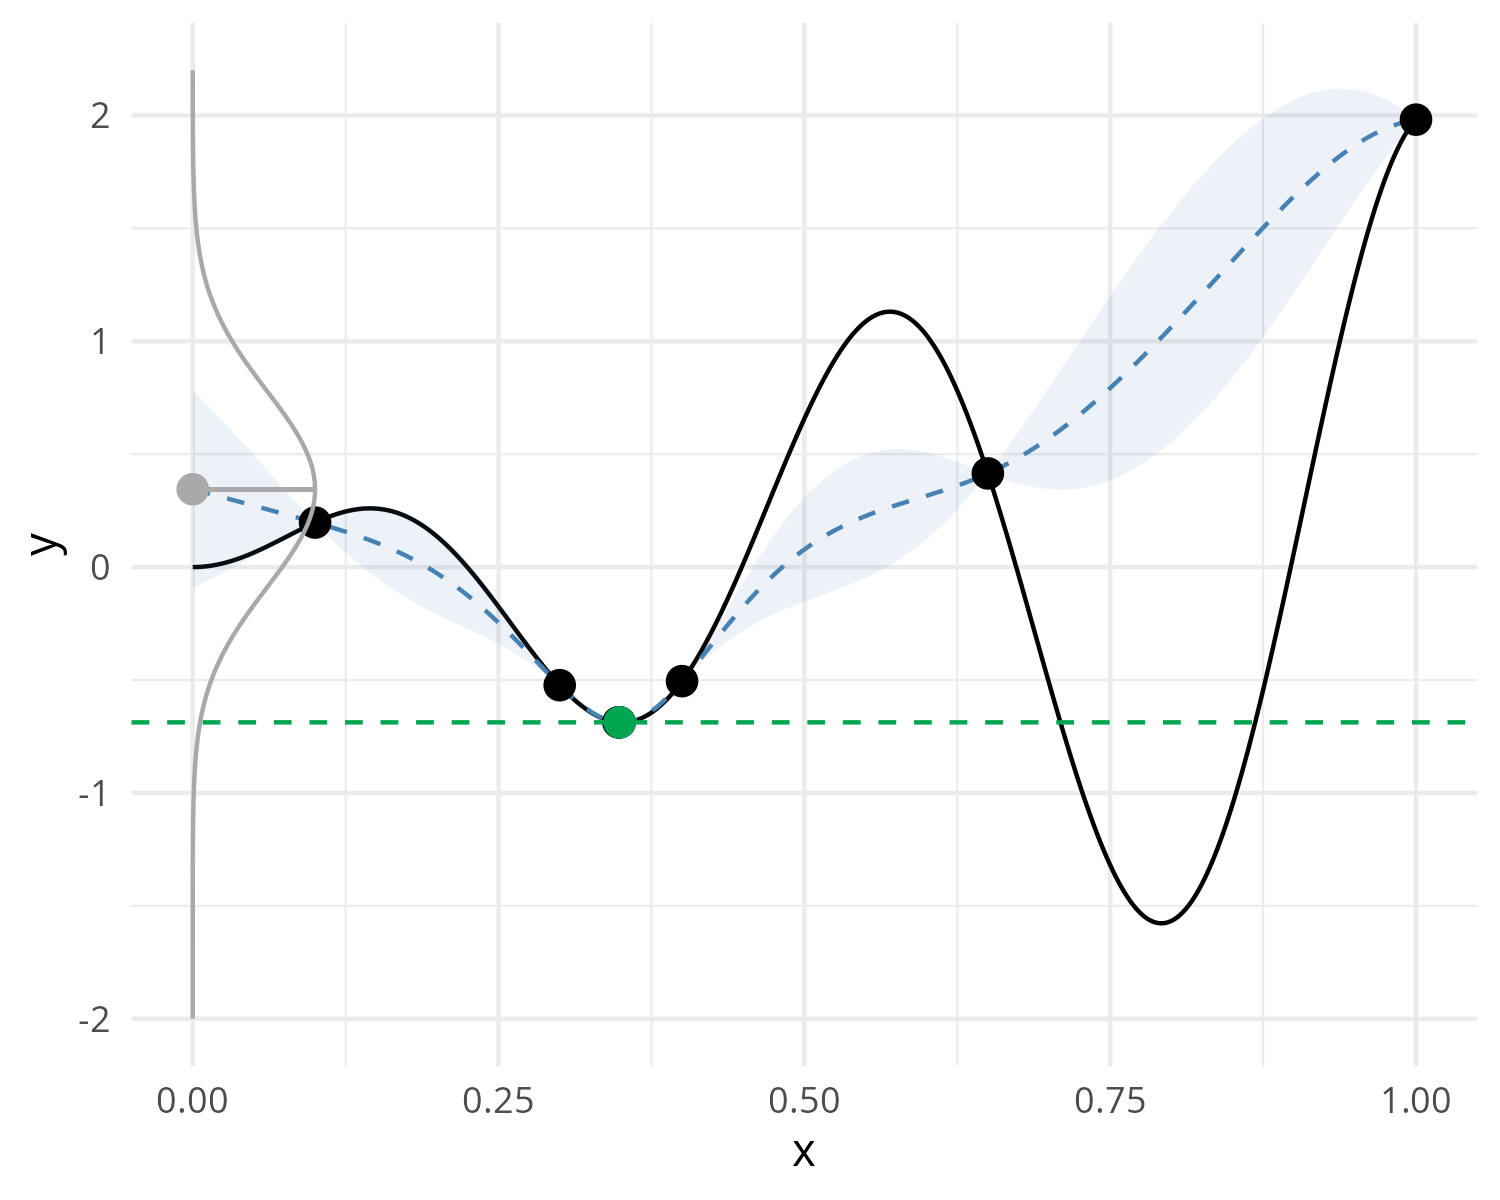
\includegraphics[width=\textwidth]{images/bayesian_loop_sm_normal_fmin.png}
        \end{center}
        \column{.5\textwidth}
        \begin{center}
            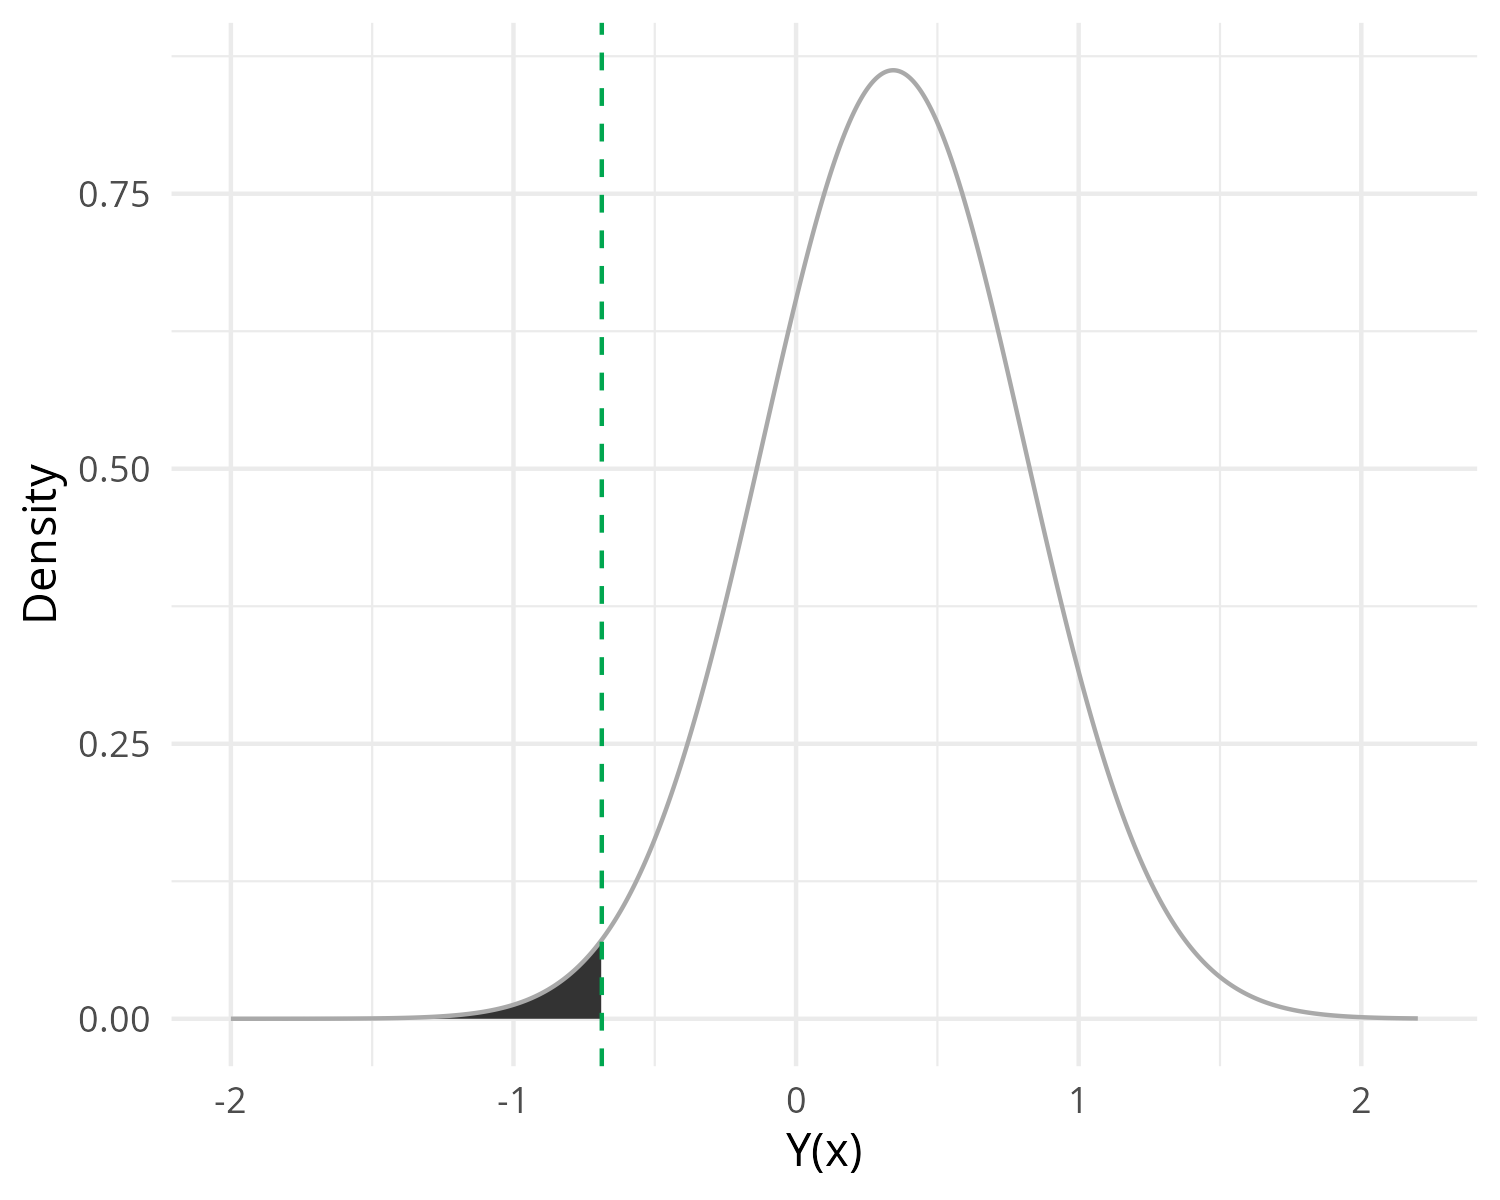
\includegraphics[width=\textwidth]{images/bayesian_loop_pi_0.png}
        \end{center}
    \end{columns}
    \footnotesize \textbf{Left:} The green vertical line represents $\fmin$. \textbf{Right:} $a_{\text{PI}}(\xv)$ is given by the black area.
\end{frame}

%----------------------------------------------------------------------

\begin{frame}{Probability of Improvement}
    \textbf{Note:} $a_\text{PI}(\xv) = 0$ for design points $\xv$, since
    \begin{itemize}
        \item $\sh(\xv) = 0$,
        \item $\surro(\xv) = \cost(\xv) \geq \fmin \;\Leftrightarrow\; \fmin - \surro(\xv) \leq 0$.
    \end{itemize}
    Therefore:
    $$\Phi\!\left(\frac{\fmin - \surro(\xv)}{\sh(\xv)}\right) = \Phi(-\infty) = 0$$
\end{frame}

%----------------------------------------------------------------------

\begin{frame}{Probability of Improvement}
    \begin{itemize}
        \item The PI does not take the size of the improvement into account
        \item Often it will propose points close to the current $\fmin$
    \end{itemize}
    We use the PI (red line) to propose the next point\ldots
    \vfill
    \begin{center}
        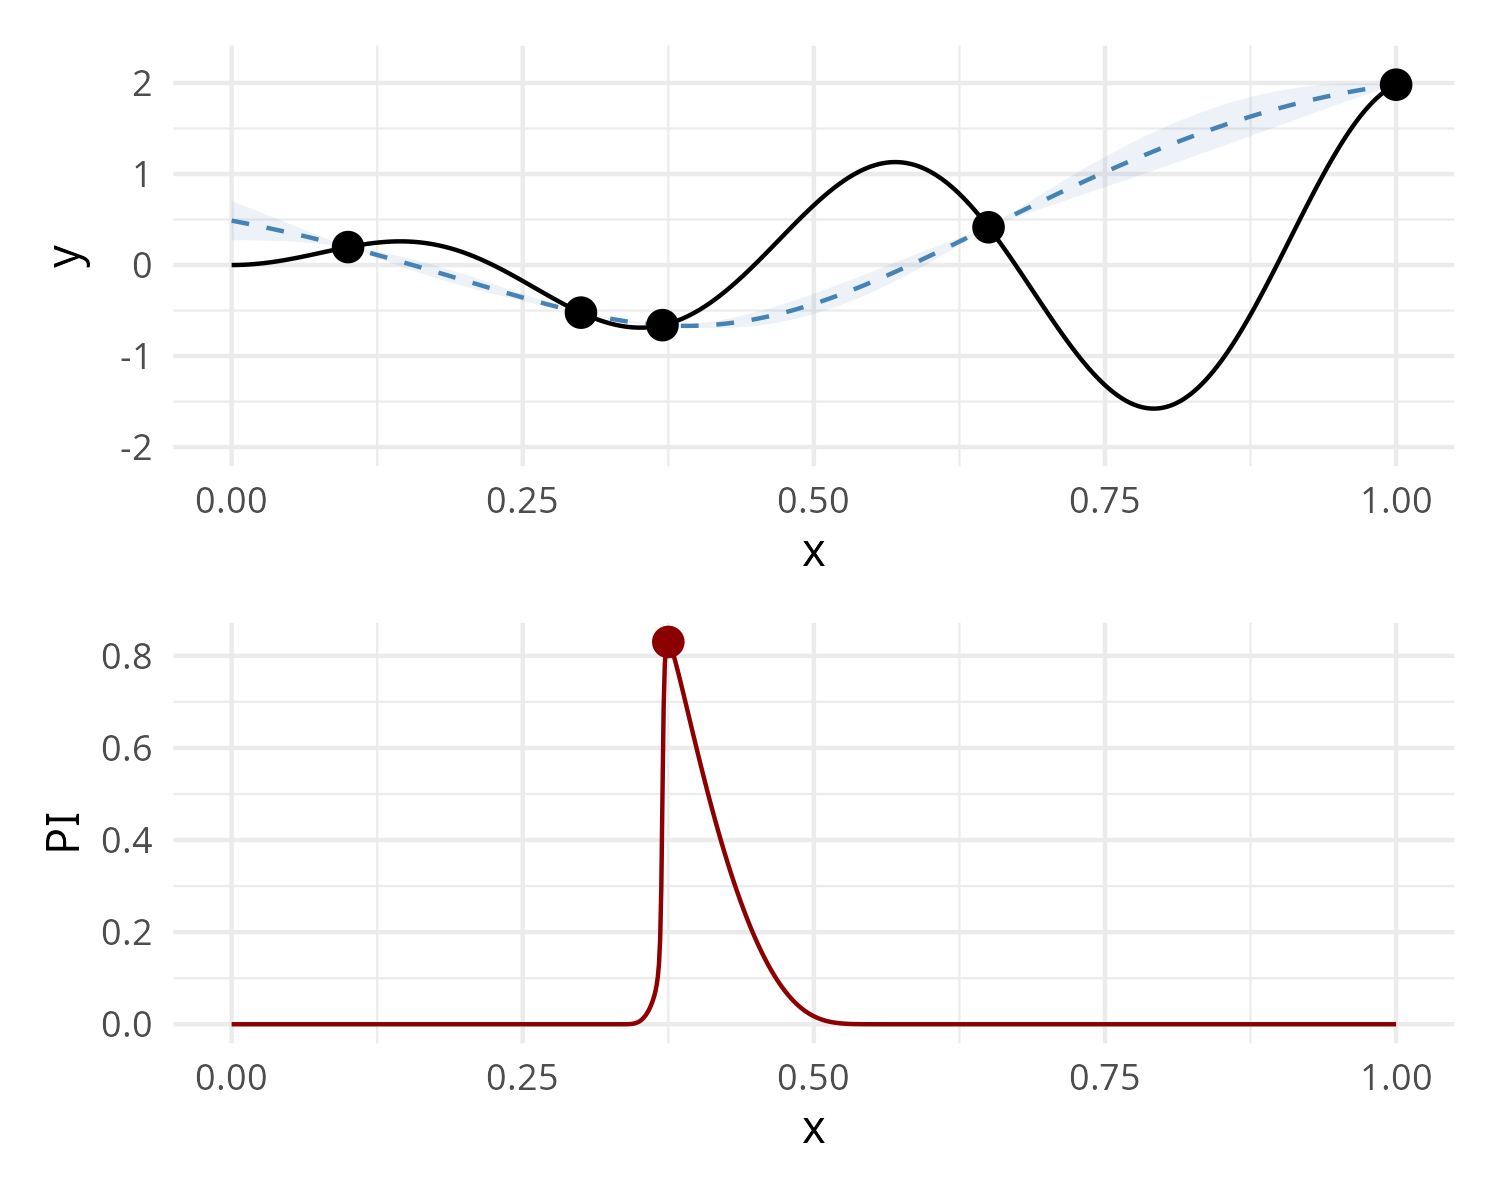
\includegraphics[width=.6\textwidth]{images/bayesian_loop_pi_1.png}
    \end{center}
    The red point depicts $\argmax_{\xv \in \pcs} a_{\text{PI}}(\xv)$.
\end{frame}

%----------------------------------------------------------------------

\begin{frame}{Probability of Improvement}
    \ldots evaluate that point, refit the SM and propose the next point.
    \vfill
    \begin{center}
        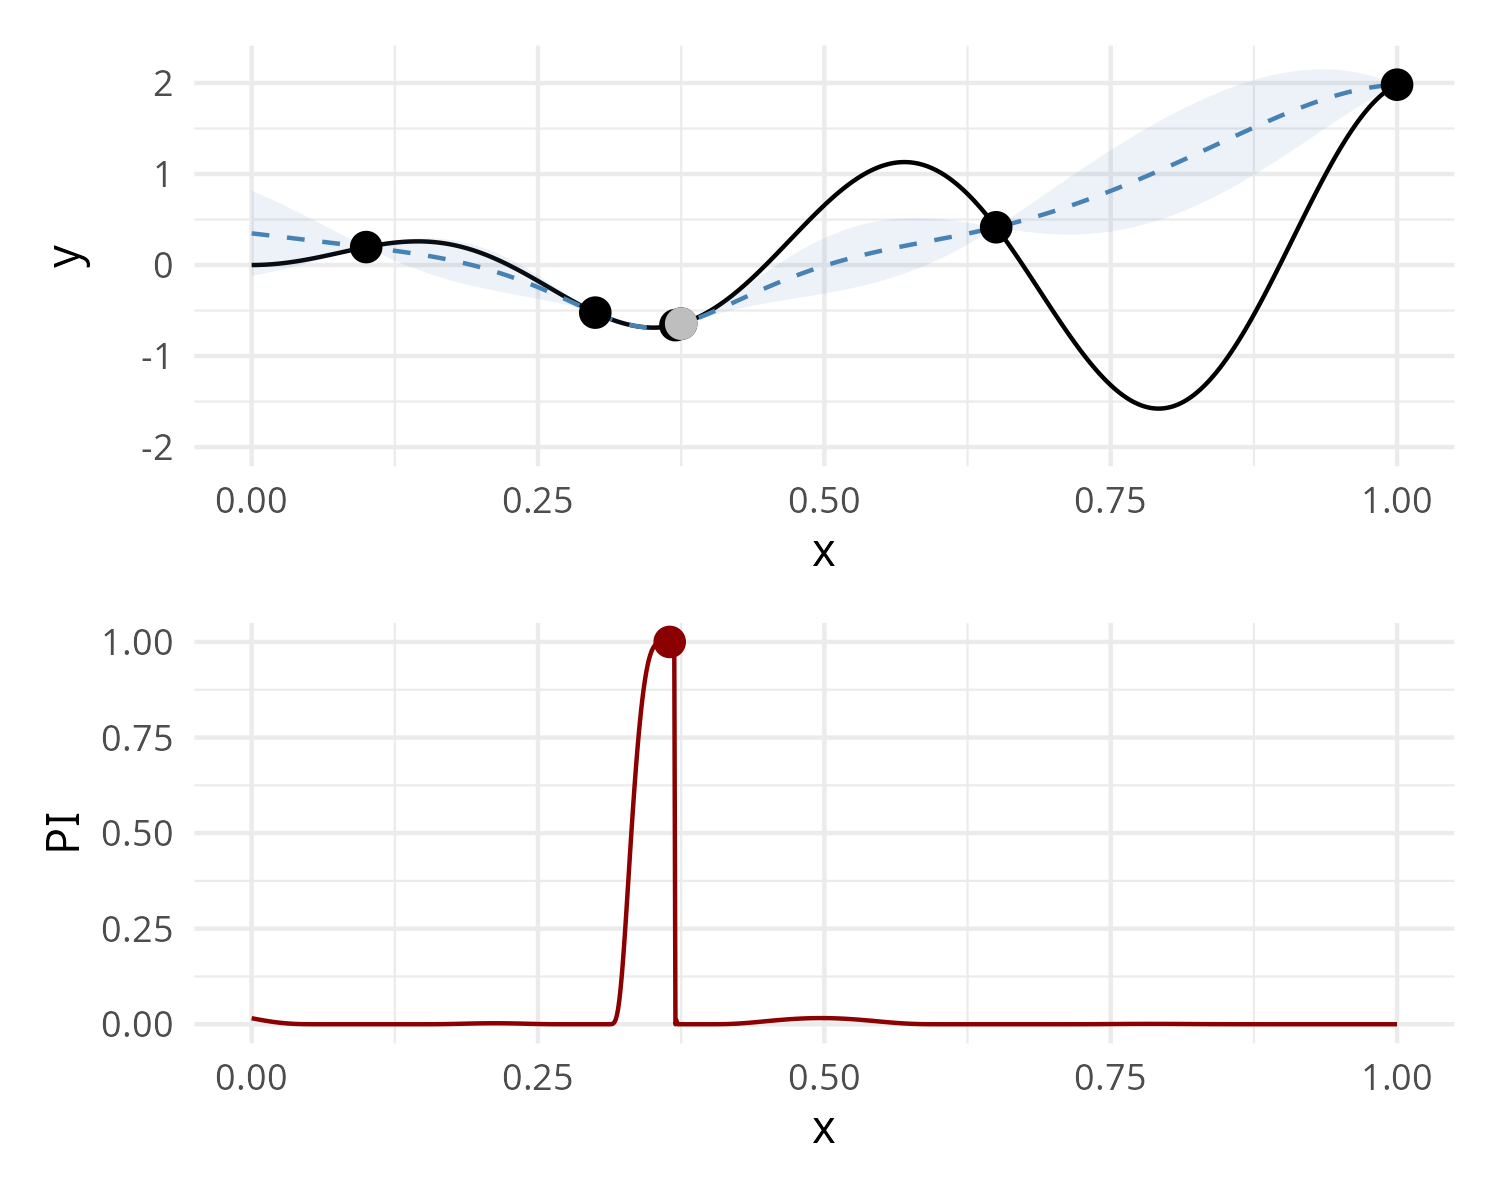
\includegraphics[width=.7\textwidth]{images/bayesian_loop_pi_2.png}
    \end{center}
    (grey point = previous point from last iteration)
\end{frame}

%----------------------------------------------------------------------

\begin{frame}{Probability of Improvement}
    \ldots
    \vfill
    \begin{center}
        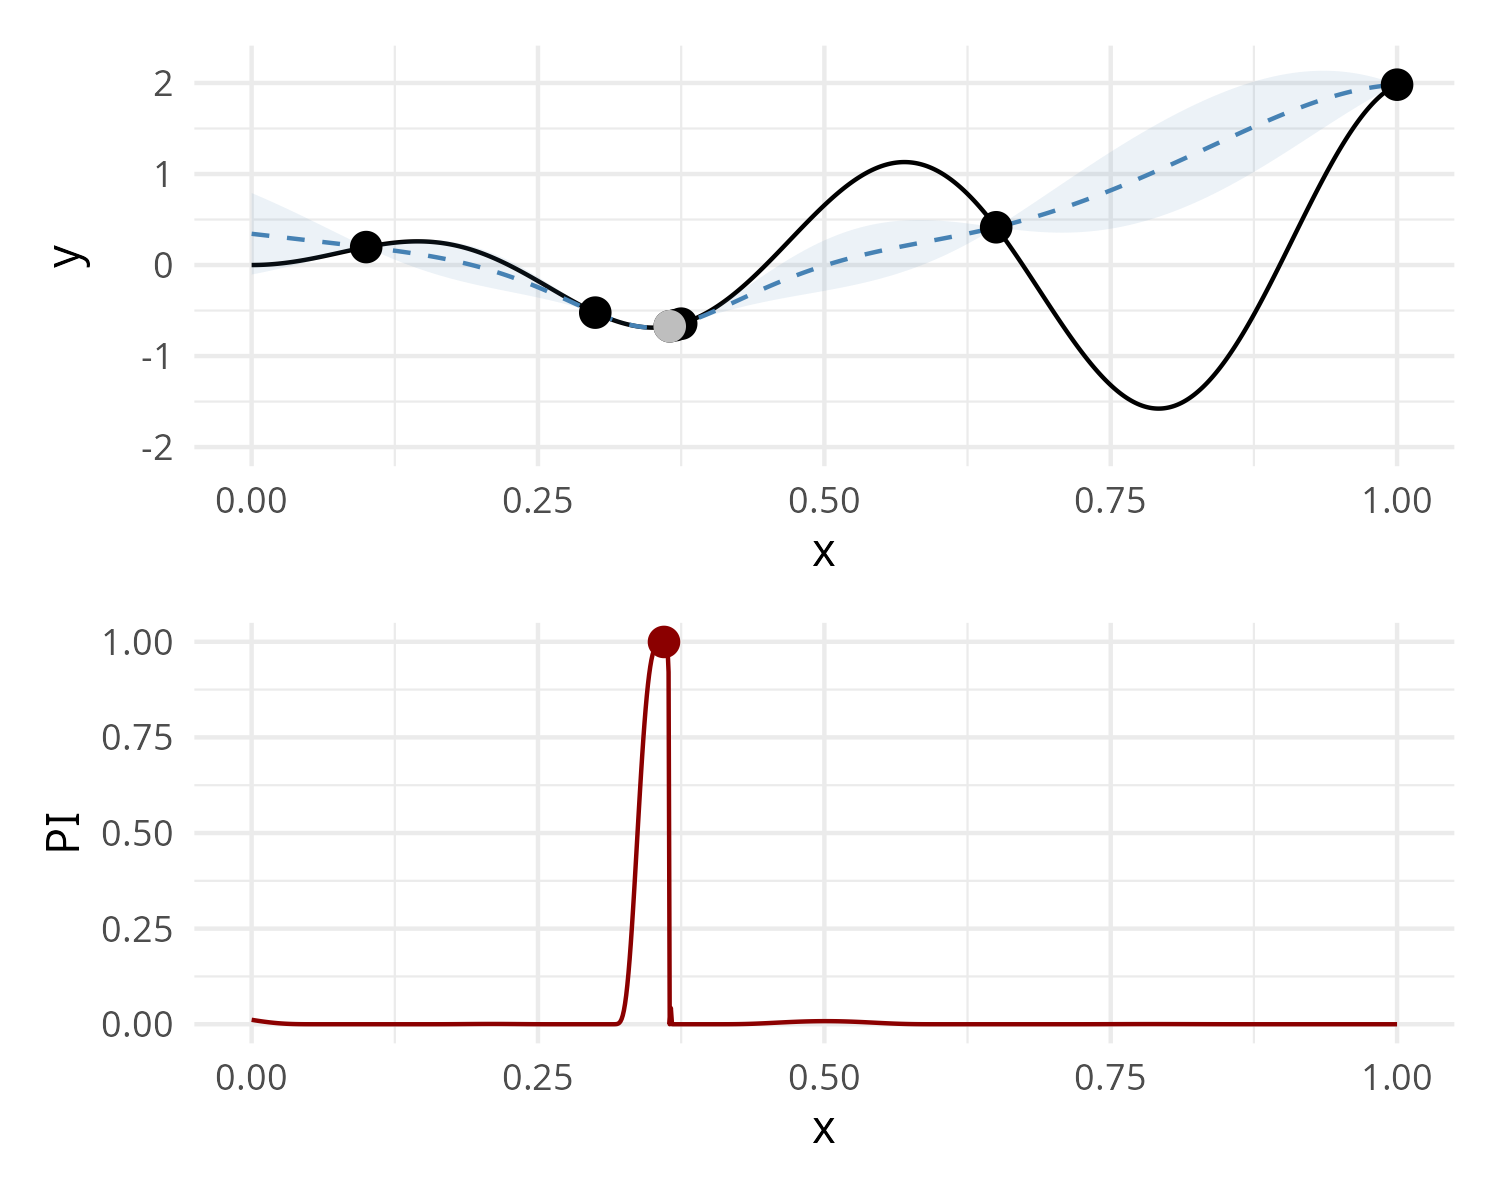
\includegraphics[width=.7\textwidth]{images/bayesian_loop_pi_3.png}
    \end{center}
\end{frame}

%----------------------------------------------------------------------

\begin{frame}{Probability of Improvement}
    In our example, using the PI results in spending plenty of time optimizing the local optimum\ldots
    \vfill
    \begin{center}
        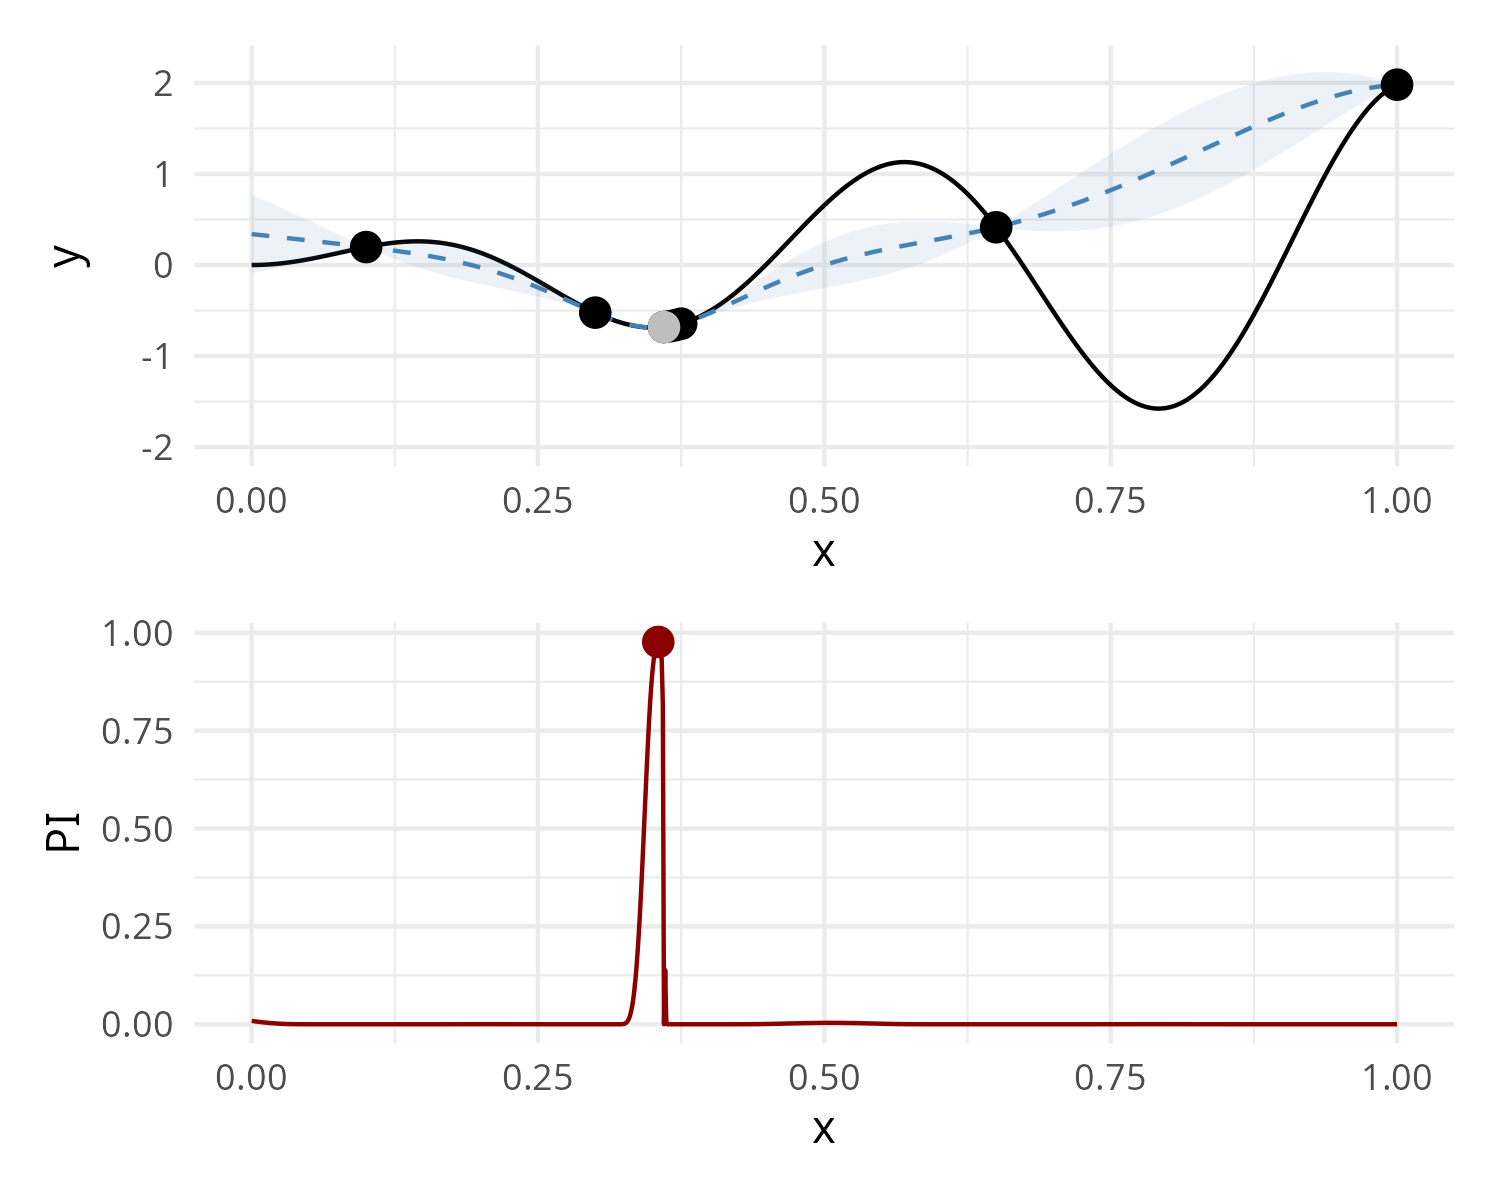
\includegraphics[width=.7\textwidth]{images/bayesian_loop_pi_4.png}
    \end{center}
\end{frame}

%----------------------------------------------------------------------

\begin{frame}{Probability of Improvement}
    \ldots
    \vfill
    \begin{center}
        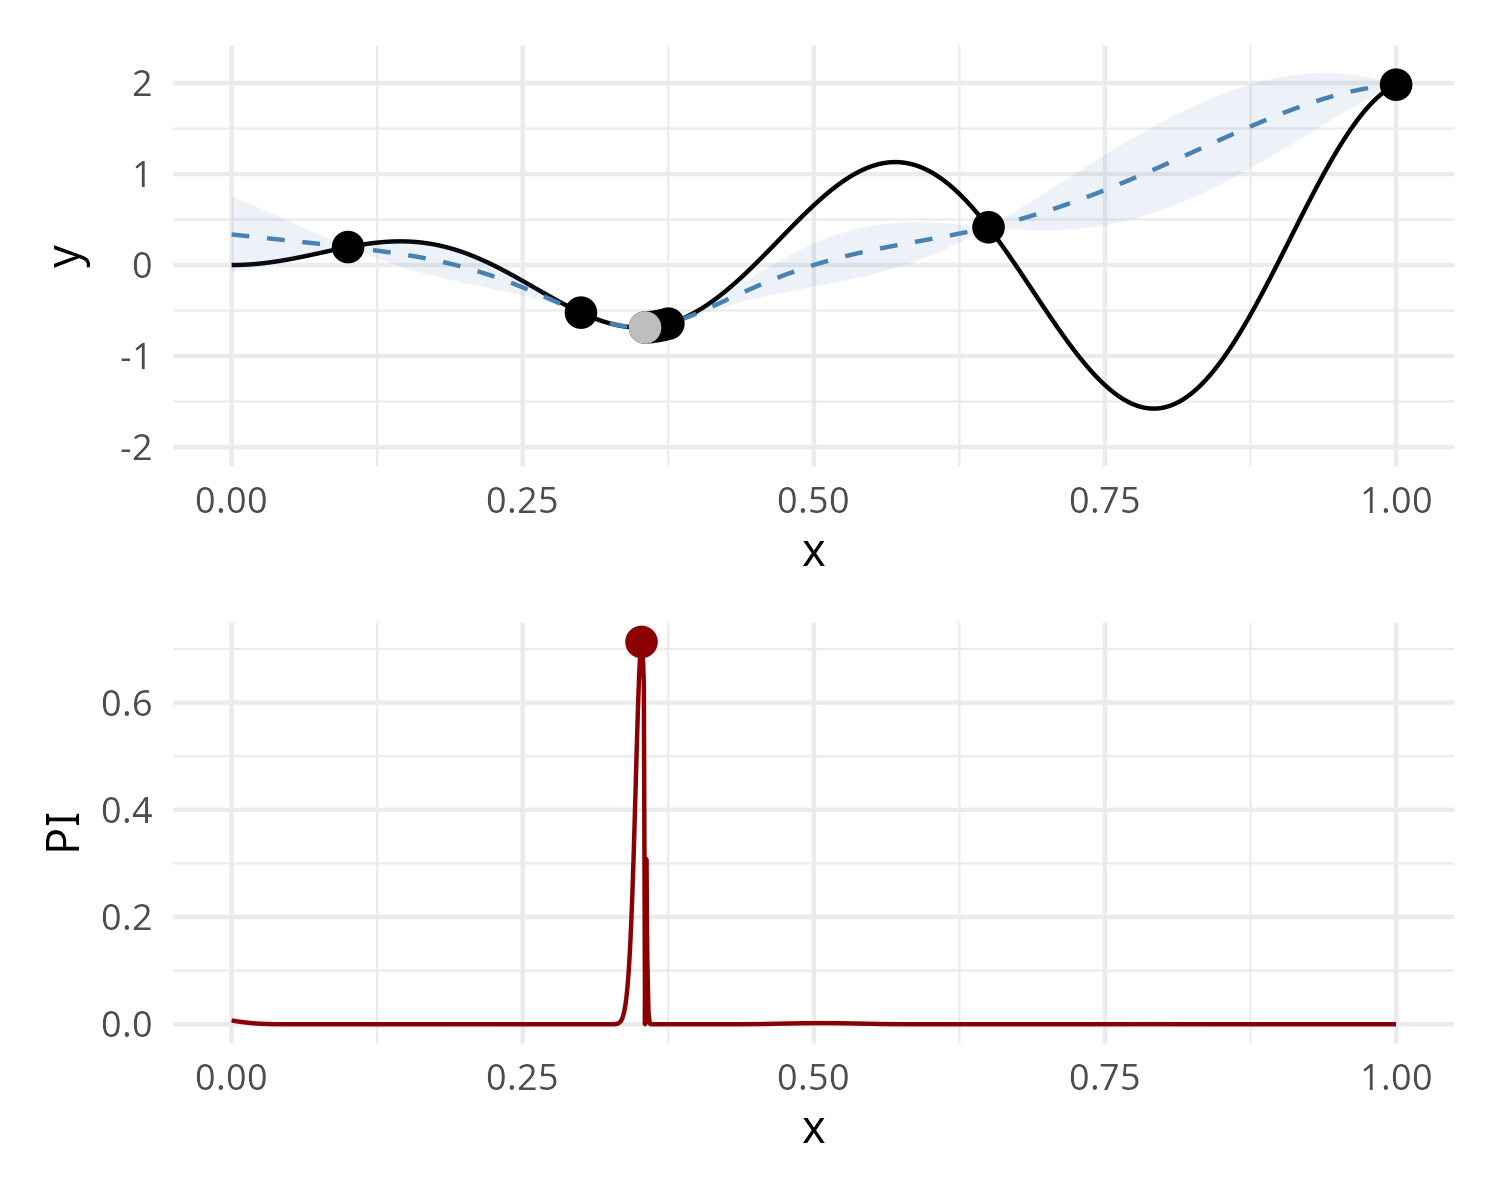
\includegraphics[width=.7\textwidth]{images/bayesian_loop_pi_5.png}
    \end{center}
\end{frame}

%----------------------------------------------------------------------

\begin{frame}{Probability of Improvement}
    \ldots
    \vfill
    \begin{center}
        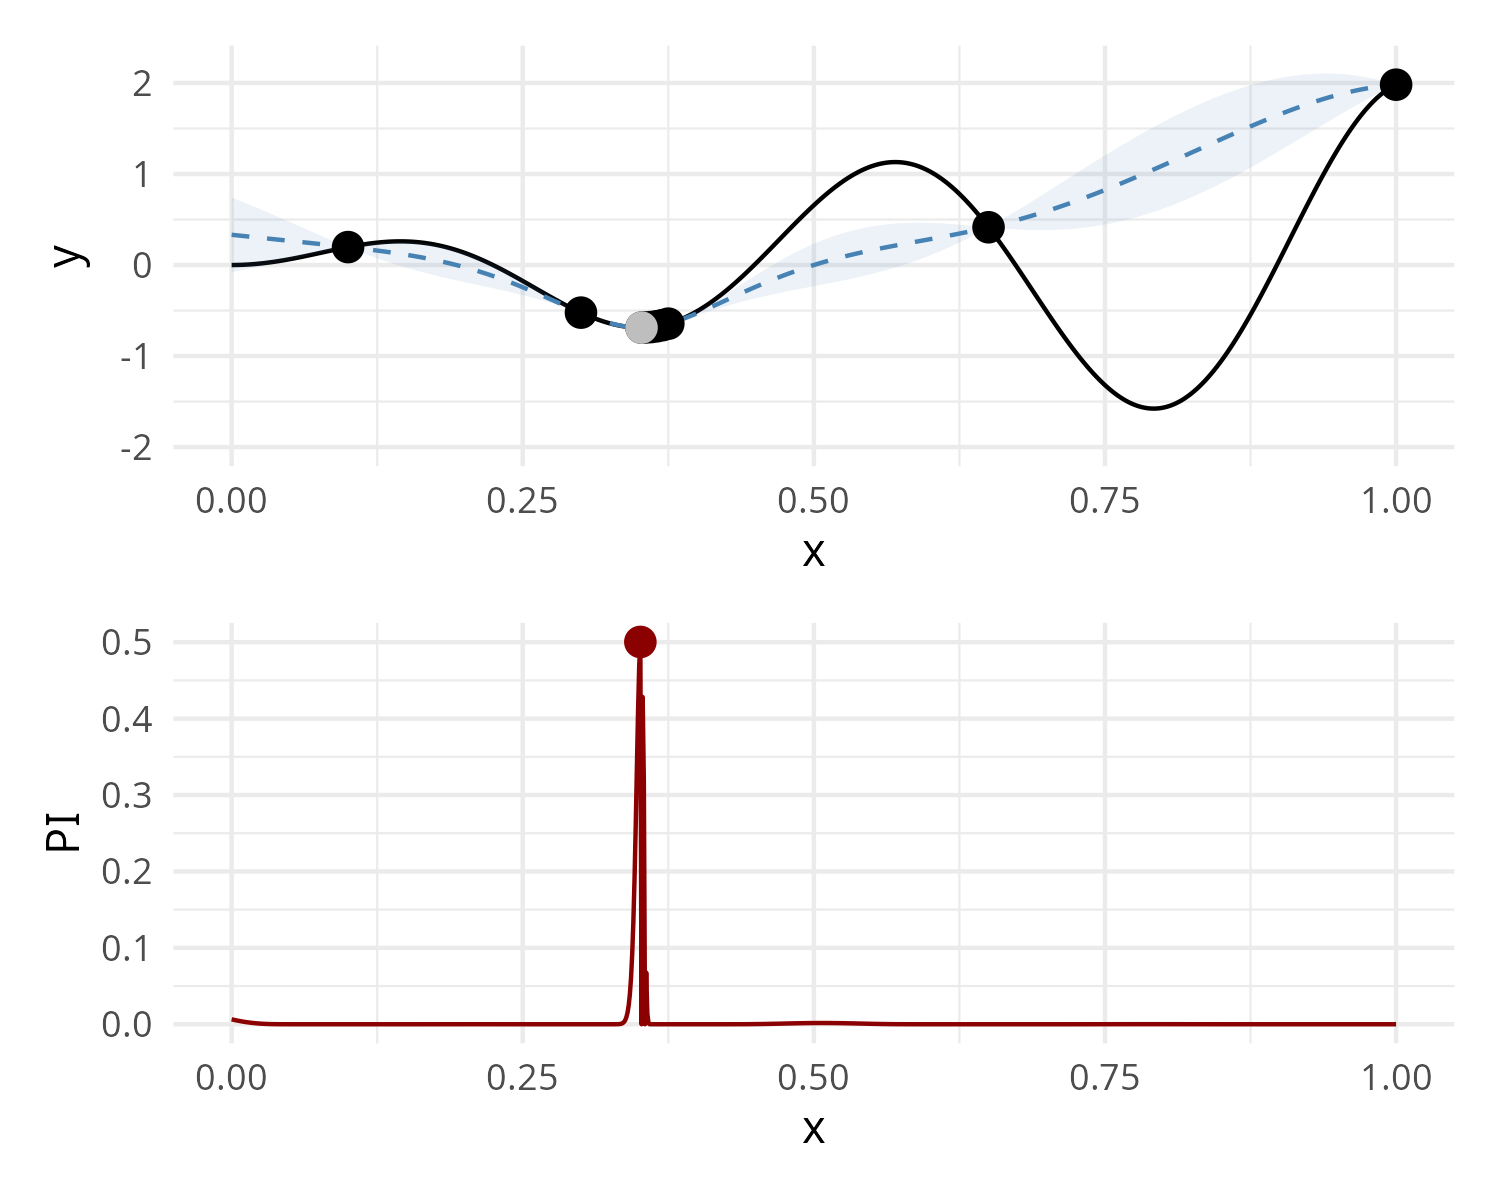
\includegraphics[width=.7\textwidth]{images/bayesian_loop_pi_6.png}
    \end{center}
\end{frame}

%----------------------------------------------------------------------

\begin{frame}{Probability of Improvement}
    \ldots
    \vfill
    \begin{center}
        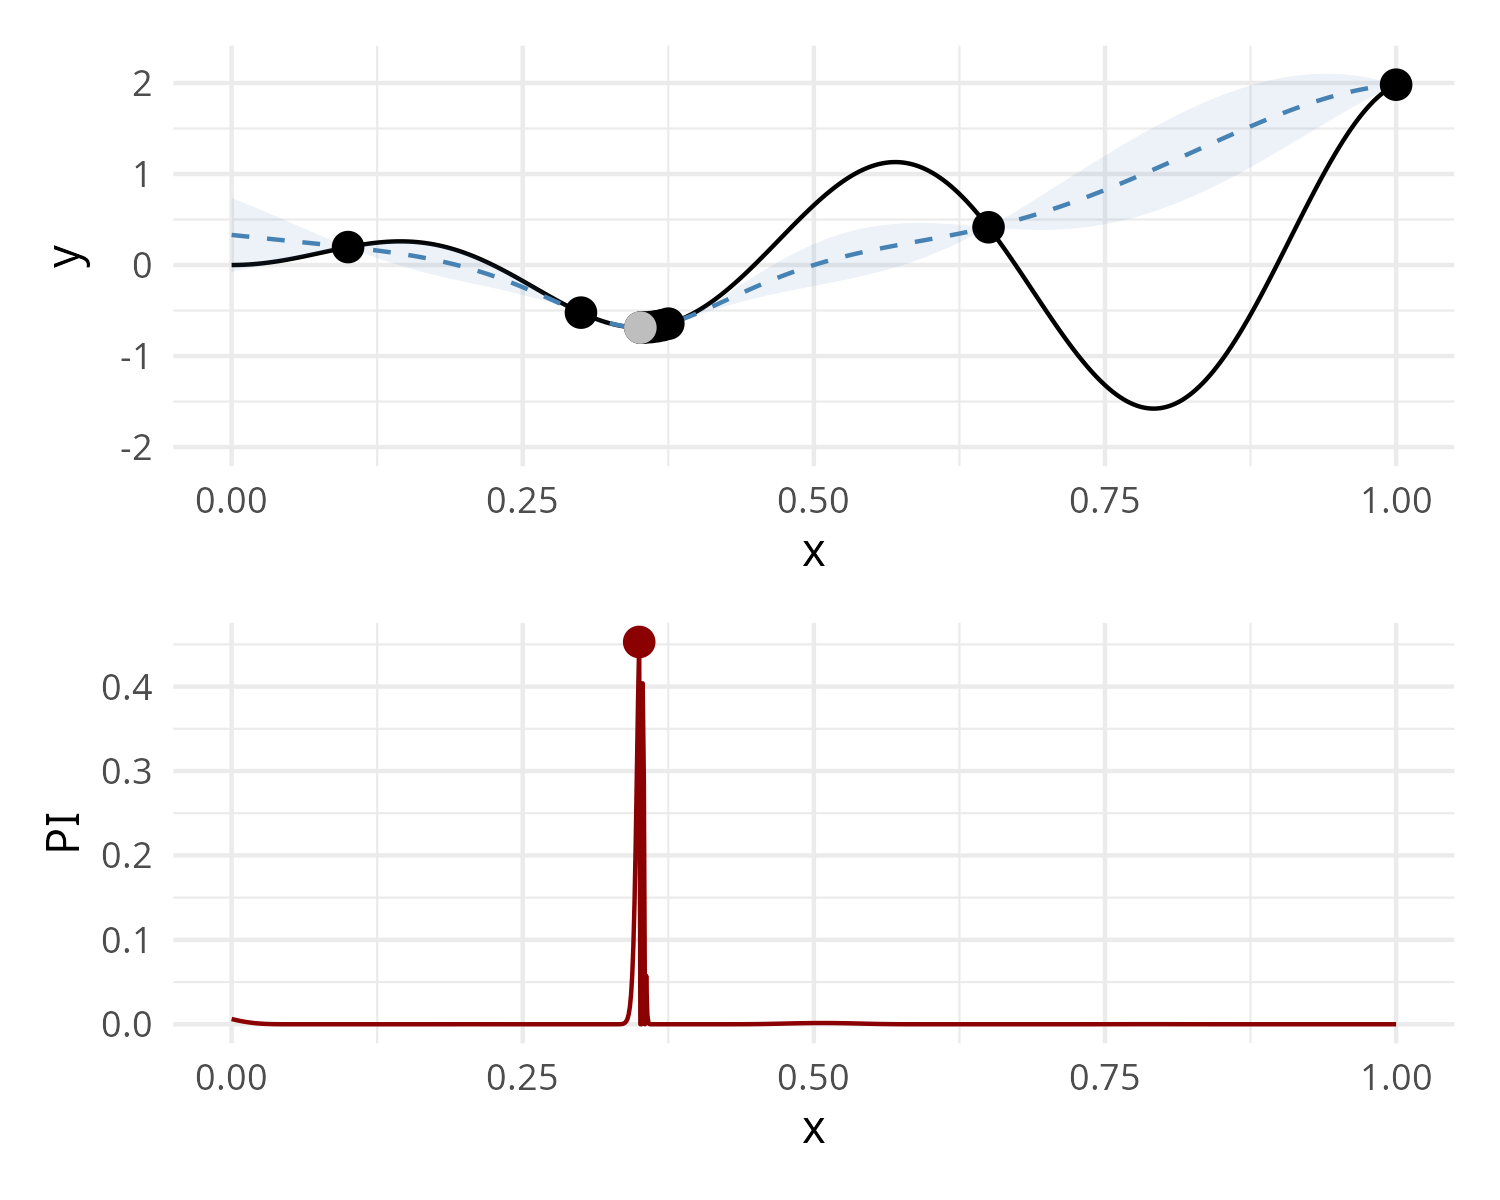
\includegraphics[width=.7\textwidth]{images/bayesian_loop_pi_7.png}
    \end{center}
\end{frame}

%----------------------------------------------------------------------

\begin{frame}{Probability of Improvement}
    \ldots eventually, we explore other regions\ldots
    \vfill
    \begin{center}
        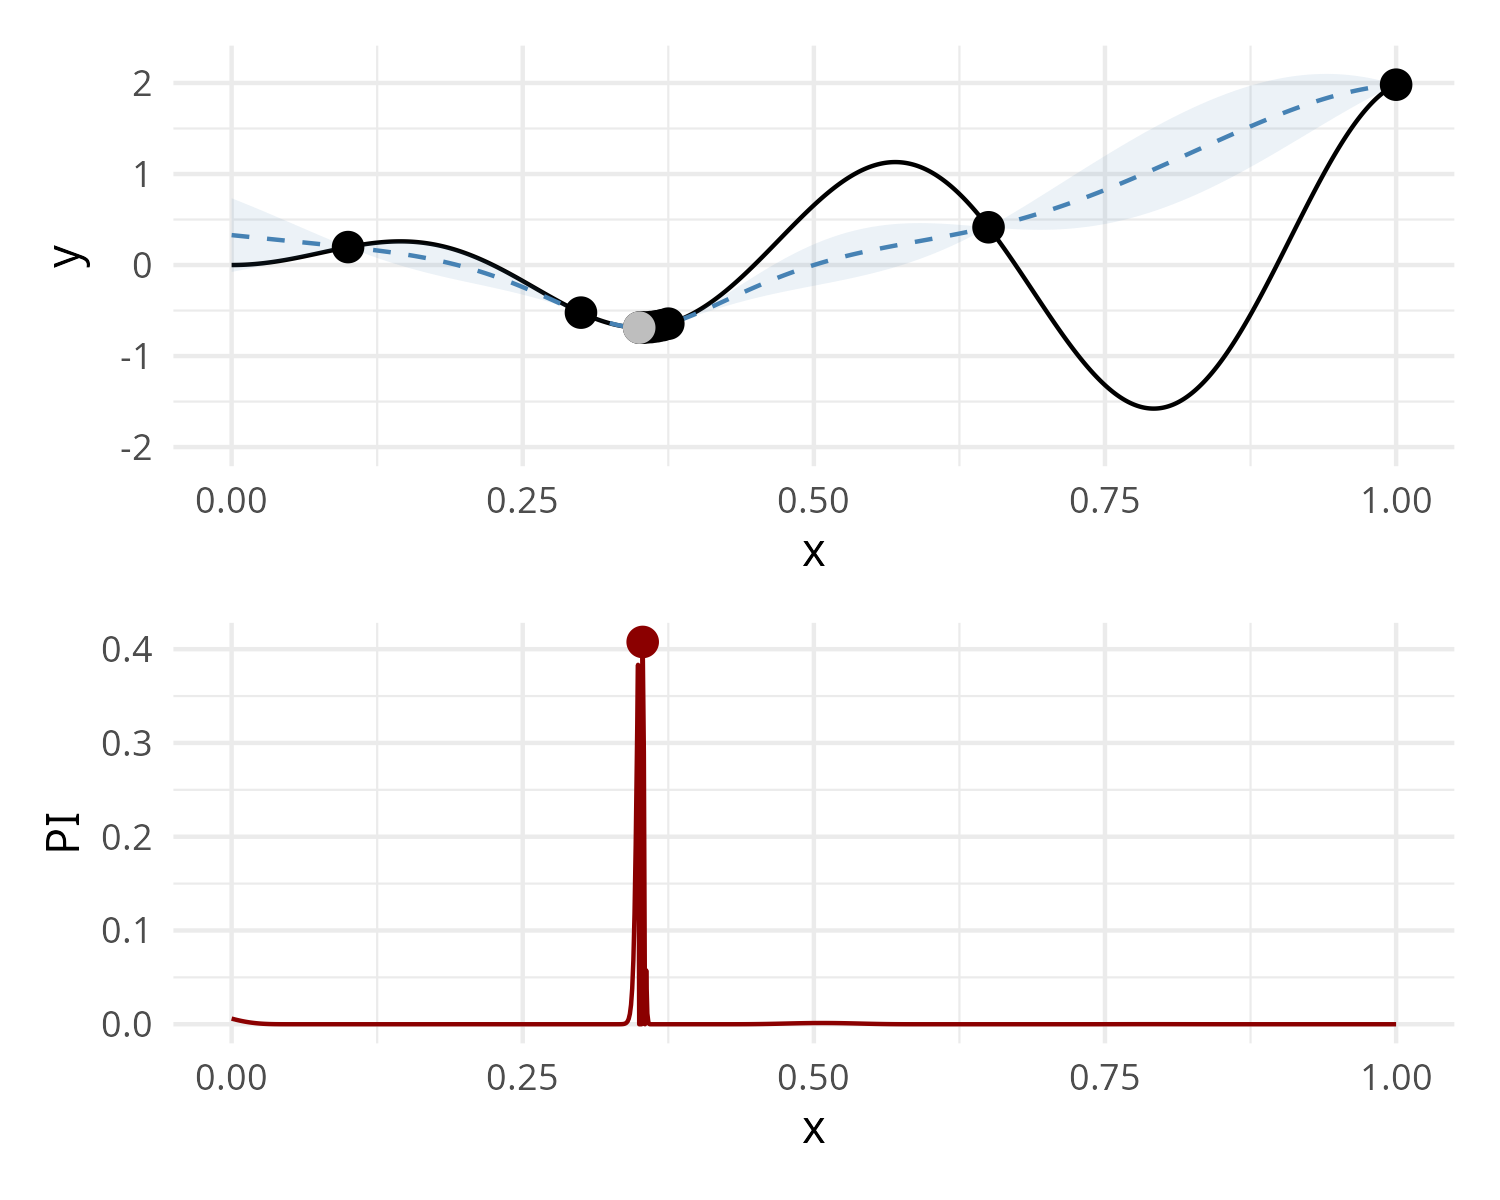
\includegraphics[width=.7\textwidth]{images/bayesian_loop_pi_8.png}
    \end{center}
\end{frame}

%----------------------------------------------------------------------

\begin{frame}{Probability of Improvement}
    \ldots
    \vfill
    \begin{center}
        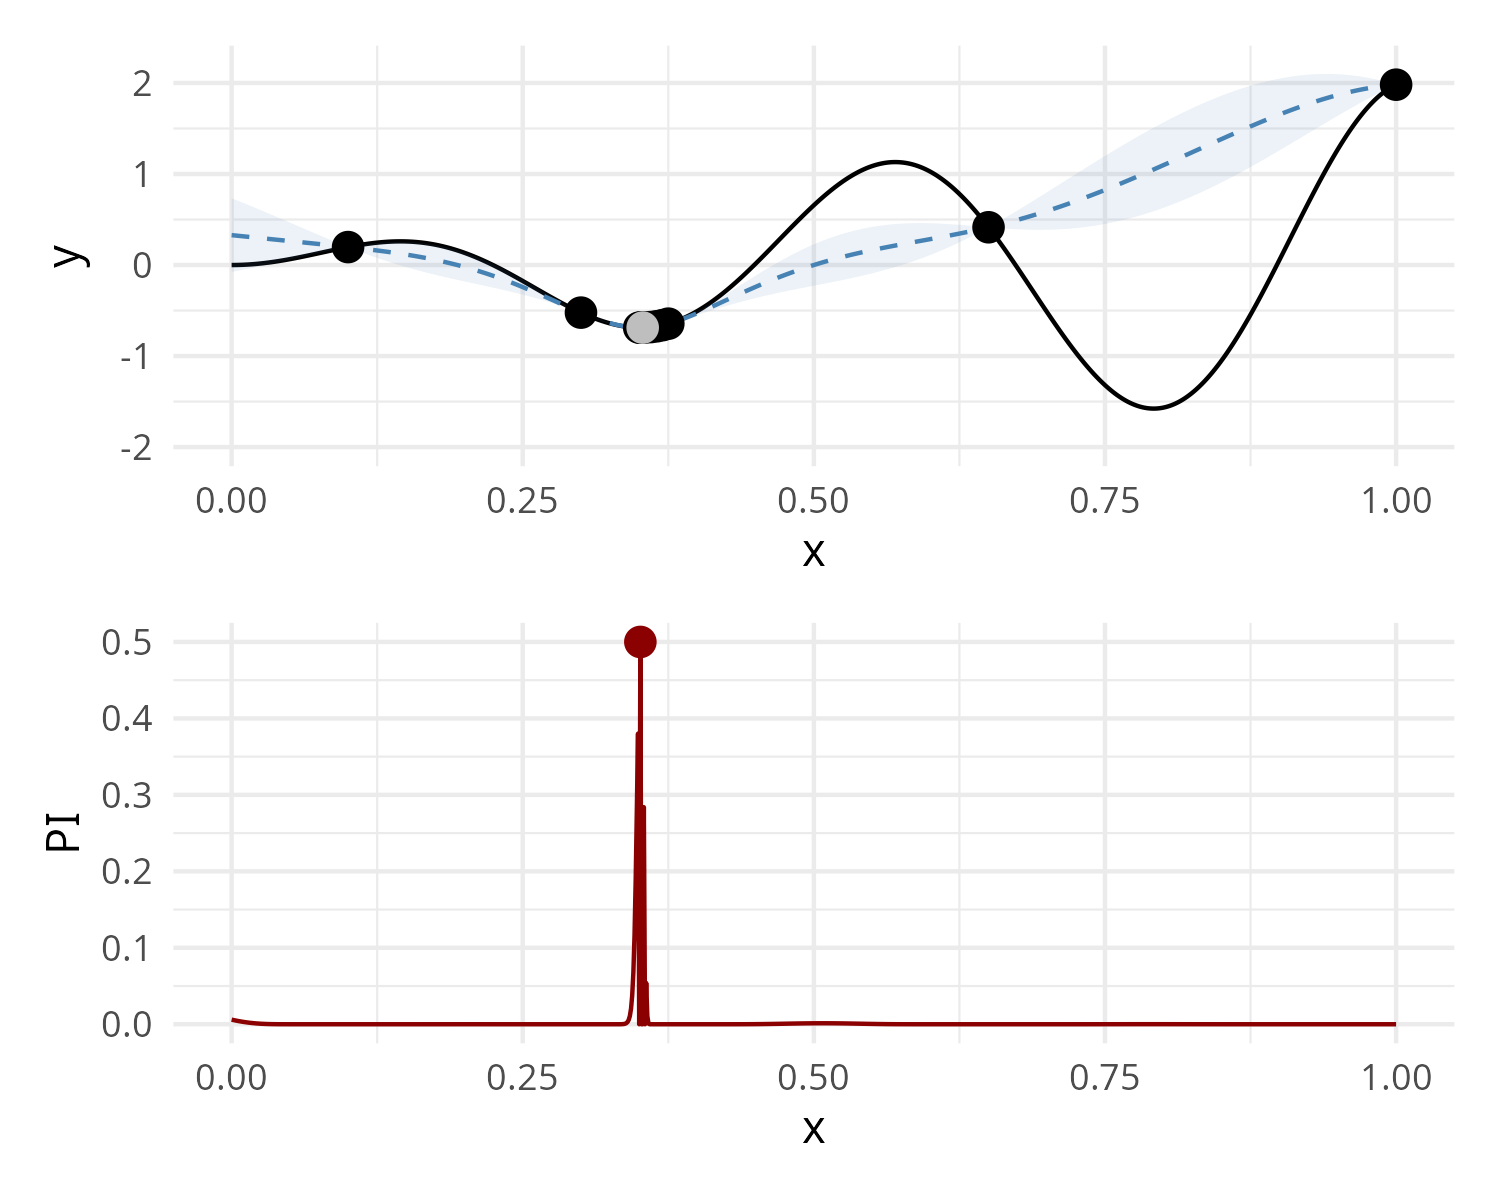
\includegraphics[width=.7\textwidth]{images/bayesian_loop_pi_9.png}
    \end{center}
\end{frame}

%----------------------------------------------------------------------

\begin{frame}{Expected Improvement}
    \textbf{Goal:} Propose $\xvsi[t+1]$ that maximizes the \textbf{Expected Improvement} (EI):
    $$a_{\text{EI}}(\xv) = \E(\max\{\fmin - Y(\xv), 0\})$$
    \vfill
    \begin{columns}
        \column{.5\textwidth}
        \begin{center}
            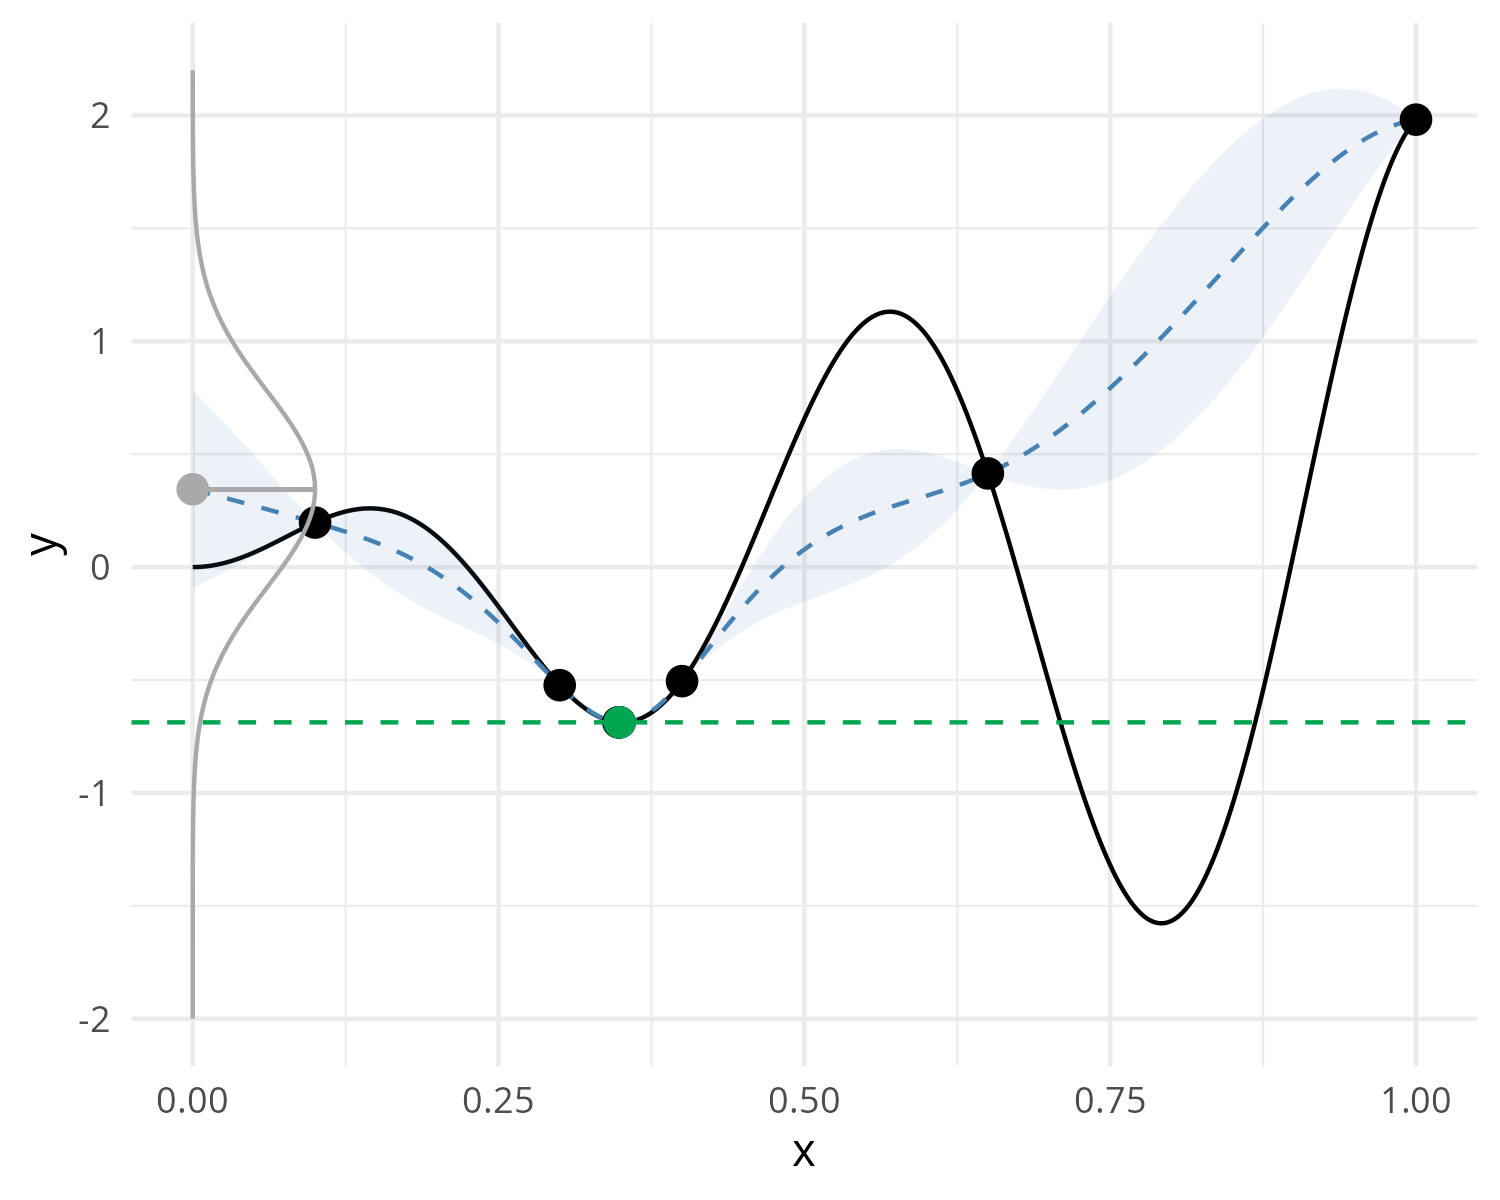
\includegraphics[width=\textwidth]{images/bayesian_loop_sm_normal_fmin.png}
        \end{center}
        \column{.5\textwidth}
        \begin{center}
            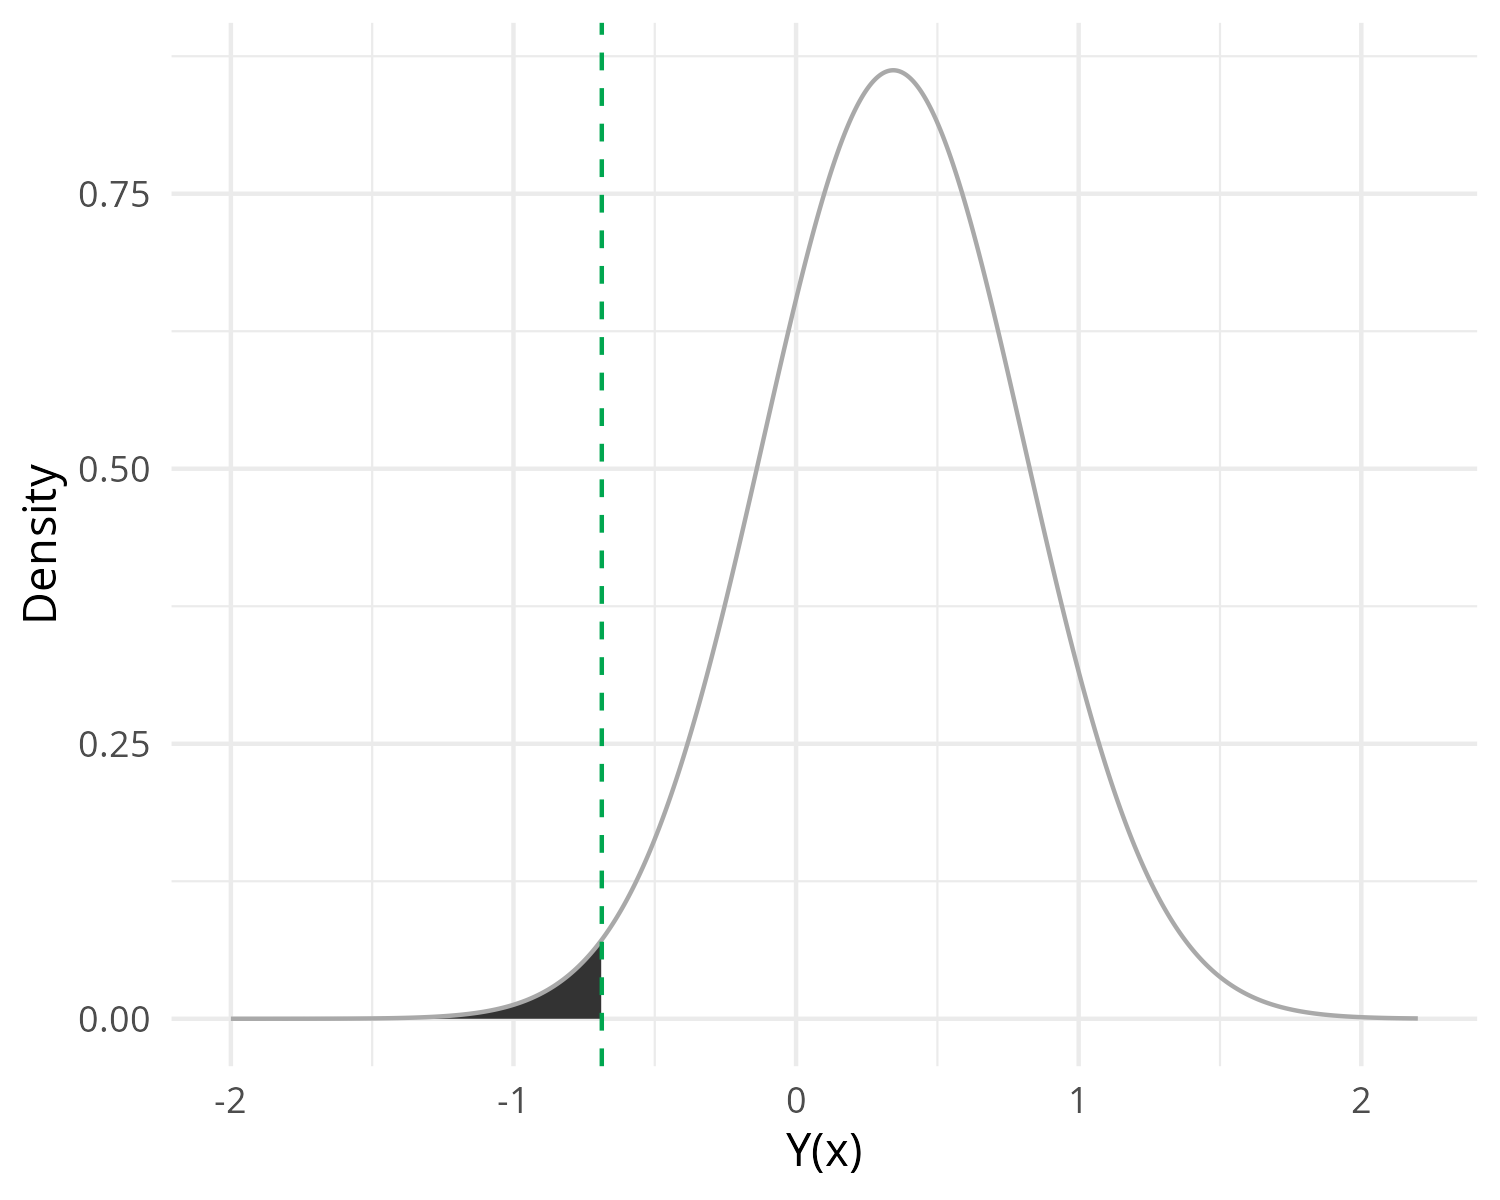
\includegraphics[width=\textwidth]{images/bayesian_loop_pi_0.png}
        \end{center}
    \end{columns}
    \vfill
    \begin{small}
    \begin{itemize}
        \item We now take the \emph{expectation} in the tail, instead of the probability as in PI
        \item Improvement is always assumed $\geq 0$
    \end{itemize}
    \end{small}
\end{frame}

%----------------------------------------------------------------------

\begin{frame}{Expected Improvement}
    If $Y(\xv) \sim \normal\left(\surro(\xv), \sh^2(\xv)\right)$, we can express the EI in closed form as:
    $$a_{\text{EI}}(\xv) = (\fmin-\surro(\xv))\, \Phi\!\left(\frac{\fmin - \surro(\xv)}{\sh(\xv)}\right) + \sh(\xv)\, \phi\!\left(\frac{\fmin - \surro(\xv)}{\sh(\xv)}\right)$$
    \begin{itemize}
        \item $a_\text{EI}(\xv) = 0$ at design points $\xv$:
        $$a_{\text{EI}}(\xv) = (\fmin-\surro(\xv)) \underbrace{\Phi\!\left(\frac{\fmin - \surro(\xv)}{\sh(\xv)}\right)}_{= 0, \text{ see PI}} + \underbrace{\sh(\xv)}_{= 0}\, \phi\!\left(\frac{\fmin - \surro(\xv)}{\sh(\xv)}\right)$$
    \end{itemize}
\end{frame}

%----------------------------------------------------------------------

\begin{frame}{Expected Improvement}
    We use the EI (red line) to propose the next point\ldots
    \vfill
    \begin{center}
        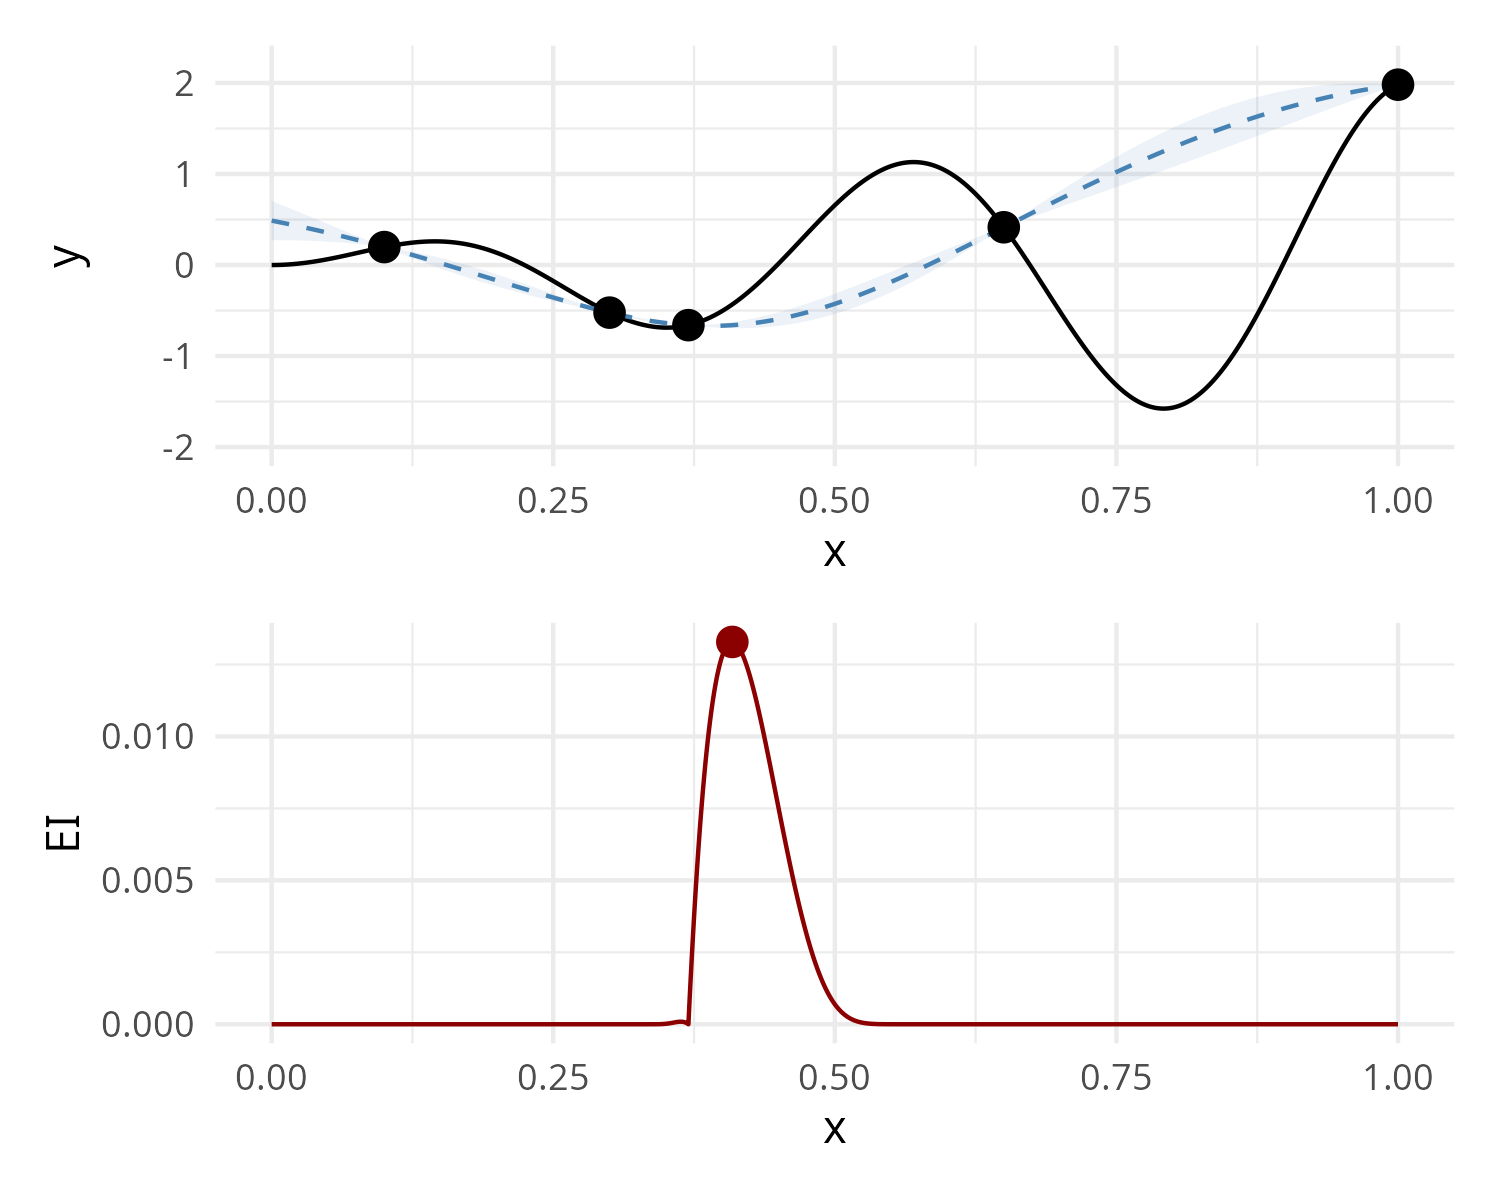
\includegraphics[width=.7\textwidth]{images/bayesian_loop_1.png}
    \end{center}
    \vfill
    The red point depicts $\argmax_{\xv \in \pcs} a_{\text{EI}}(\xv)$.
\end{frame}

%----------------------------------------------------------------------

\begin{frame}{Expected Improvement}
    \ldots evaluate that point, refit the SM and propose the next point.
    \vfill
    \begin{center}
        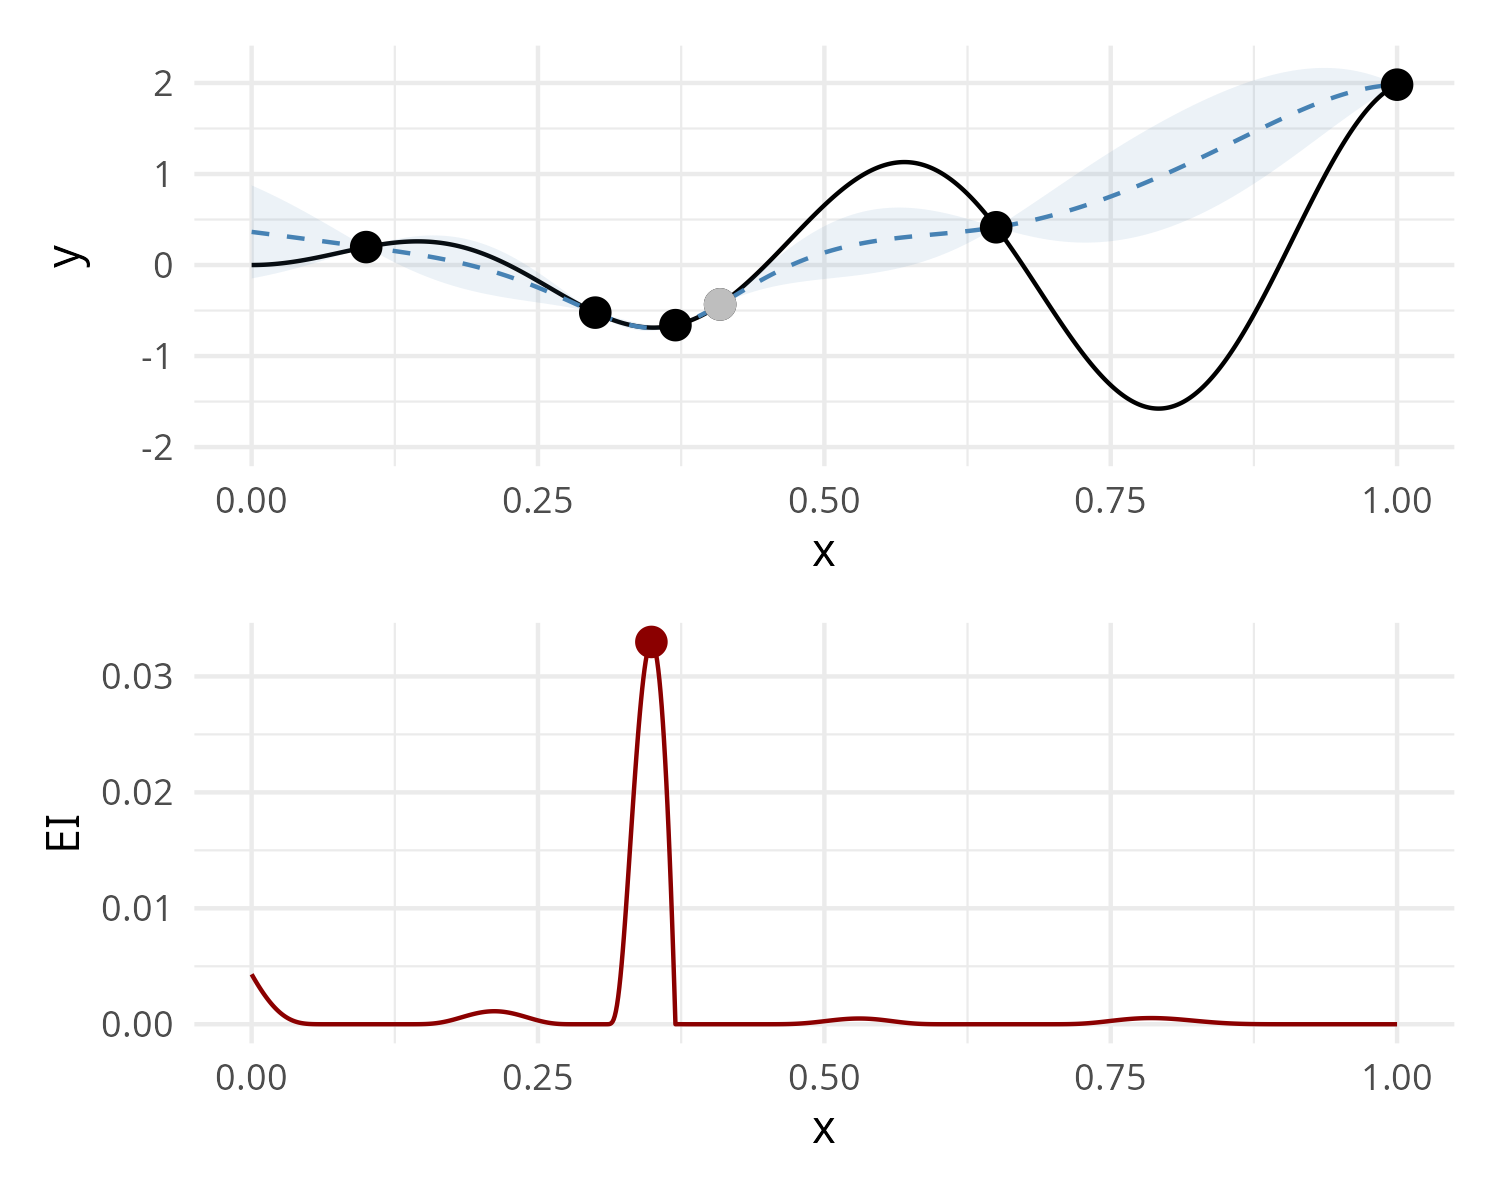
\includegraphics[width=.7\textwidth]{images/bayesian_loop_2.png}
    \end{center}
    \vfill
    (grey point = previous point from last iteration)
\end{frame}

%----------------------------------------------------------------------

\begin{frame}{Expected Improvement}
    \ldots
    \vfill
    \begin{center}
        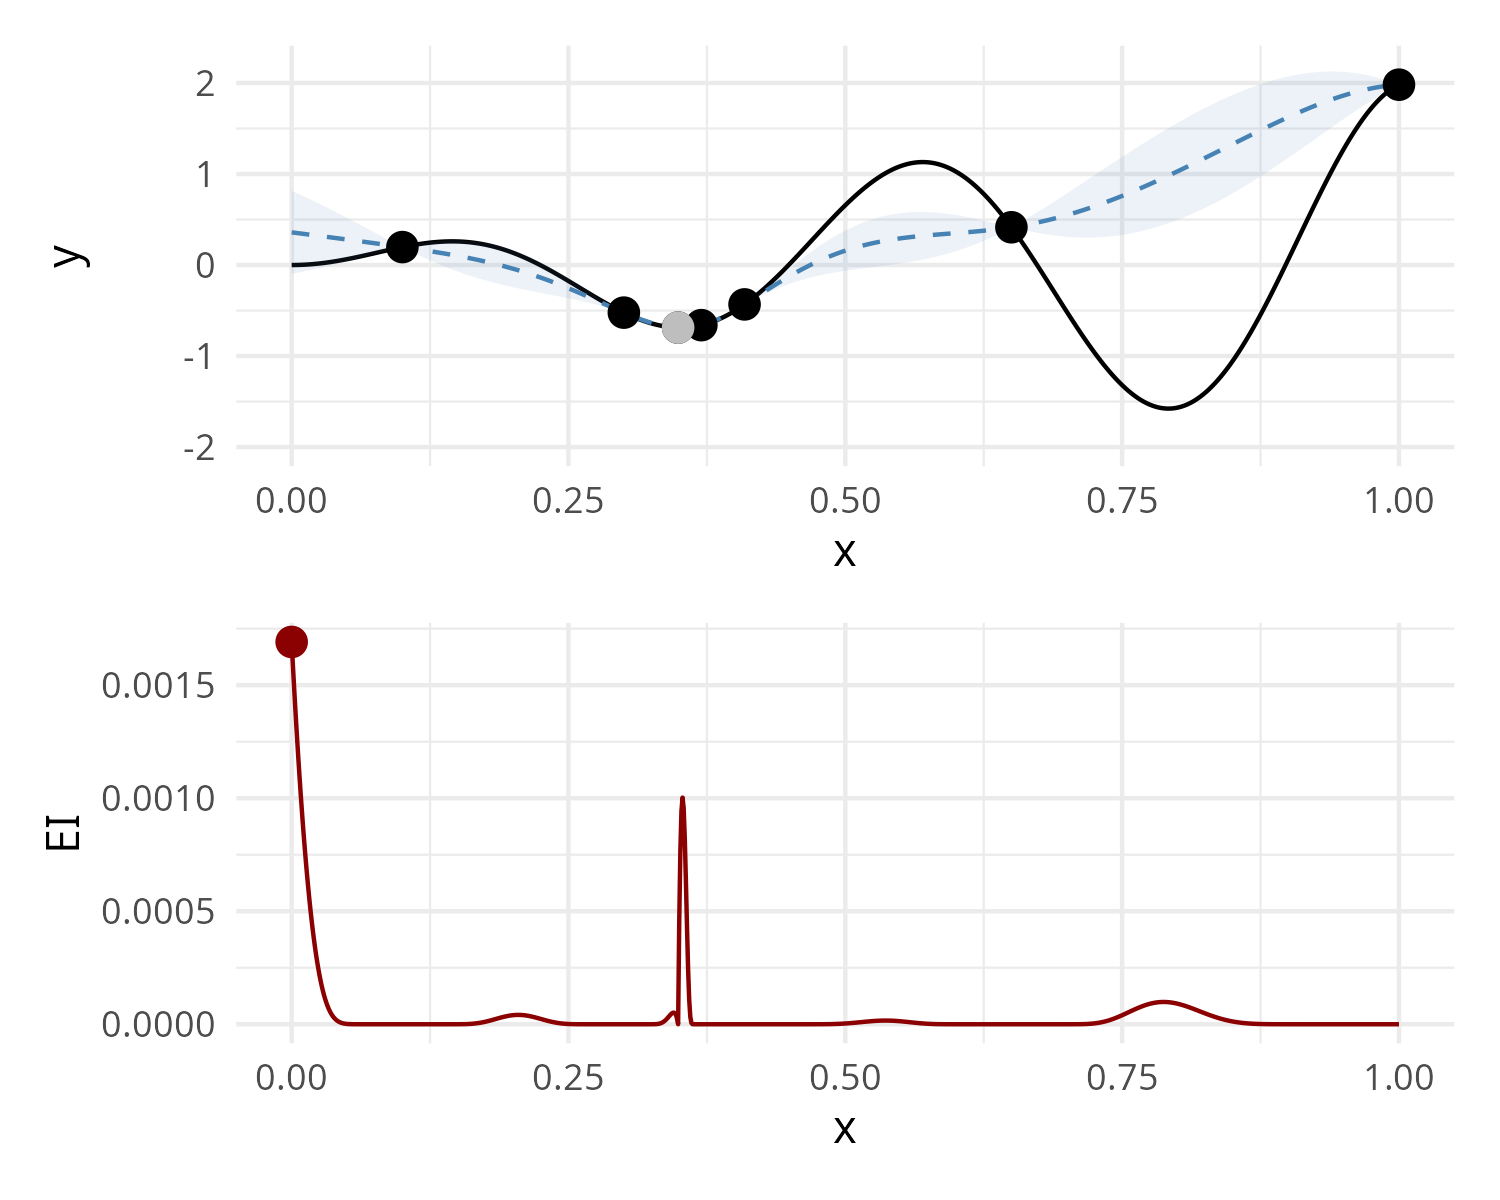
\includegraphics[width=.7\textwidth]{images/bayesian_loop_3.png}
    \end{center}
\end{frame}

%----------------------------------------------------------------------

\begin{frame}{Expected Improvement}
    \ldots
    \vfill
    \begin{center}
        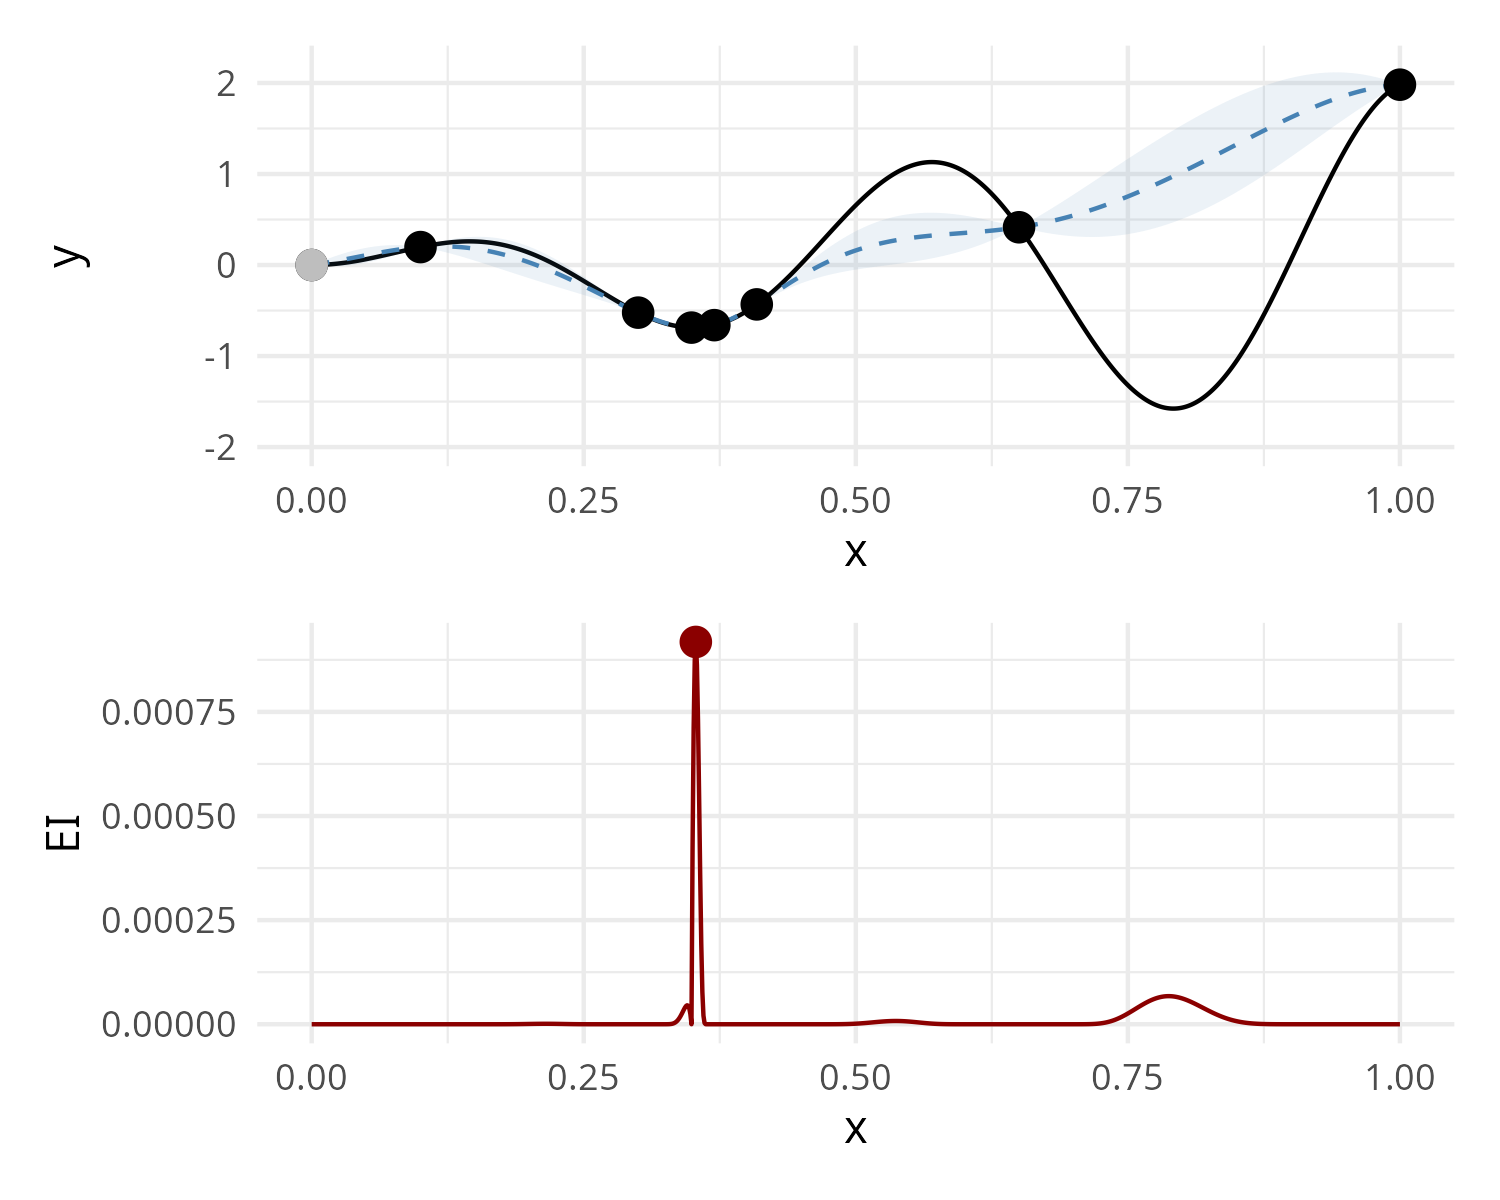
\includegraphics[width=.7\textwidth]{images/bayesian_loop_4.png}
    \end{center}
\end{frame}

%----------------------------------------------------------------------

\begin{frame}{Expected Improvement}
    \ldots
    \vfill
    \begin{center}
        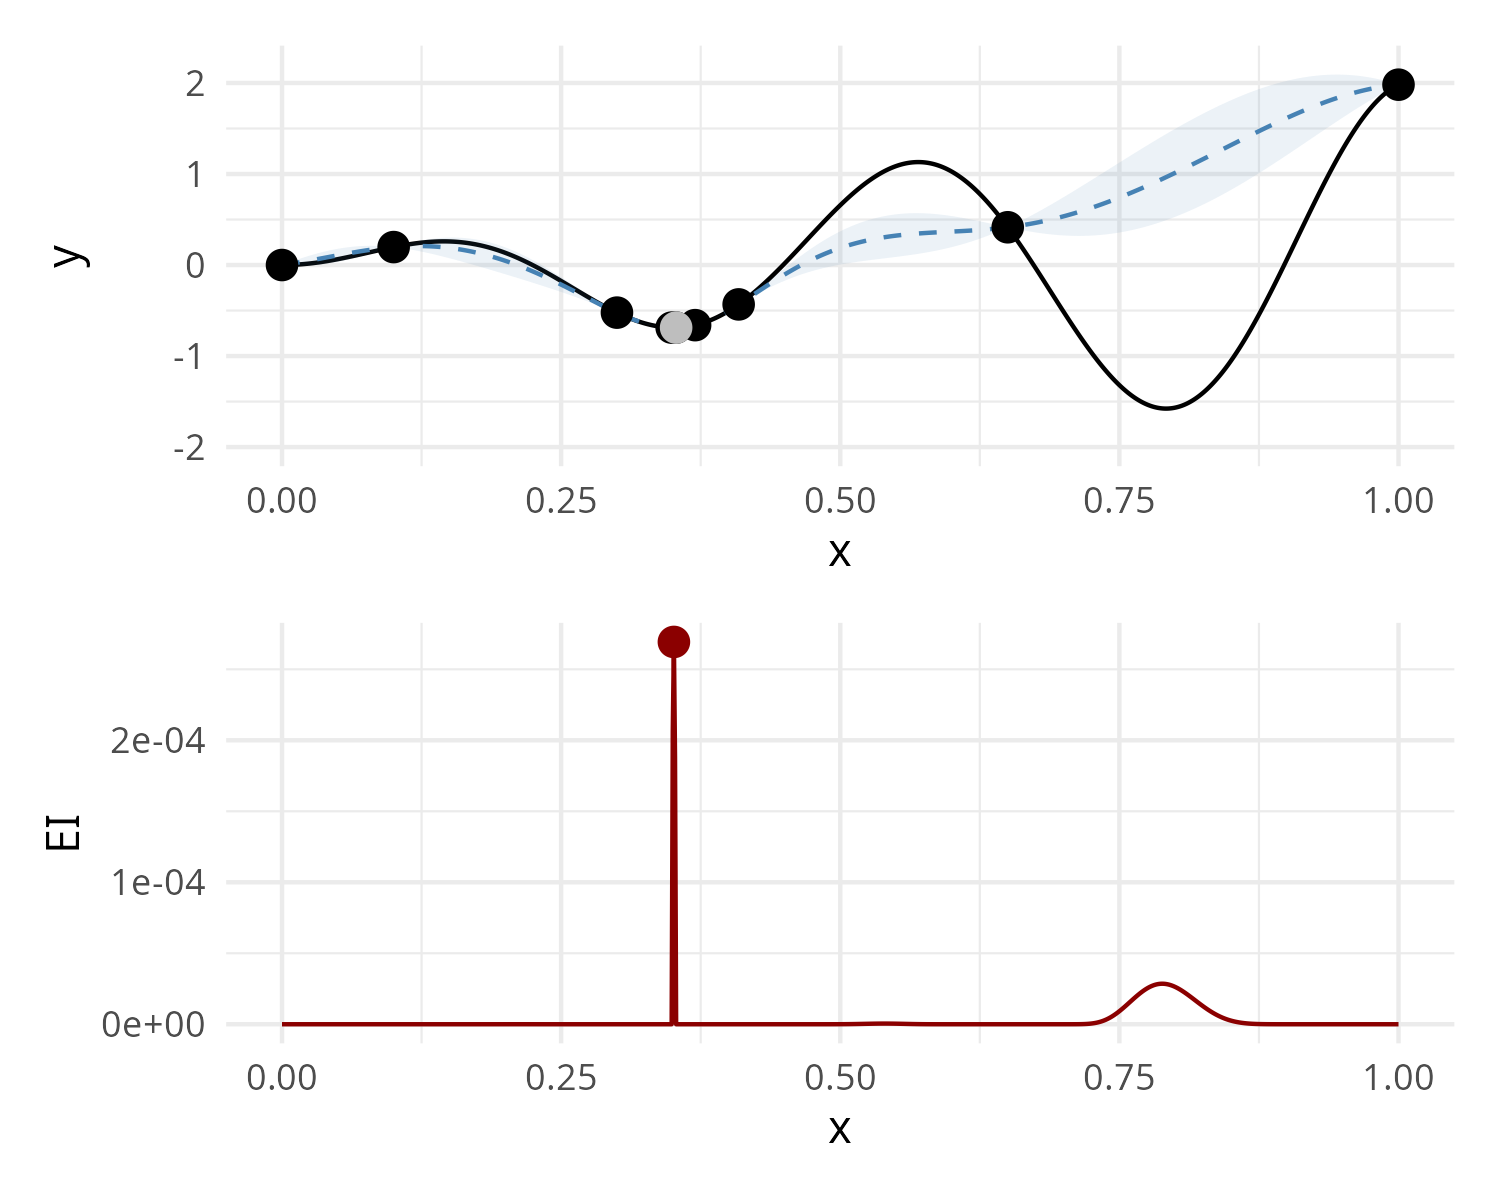
\includegraphics[width=.7\textwidth]{images/bayesian_loop_5.png}
    \end{center}
\end{frame}

%----------------------------------------------------------------------

\begin{frame}{Expected Improvement}
    The EI is capable of exploration and quickly proposes promising points in areas we have not visited yet.
    \vfill
    \begin{center}
        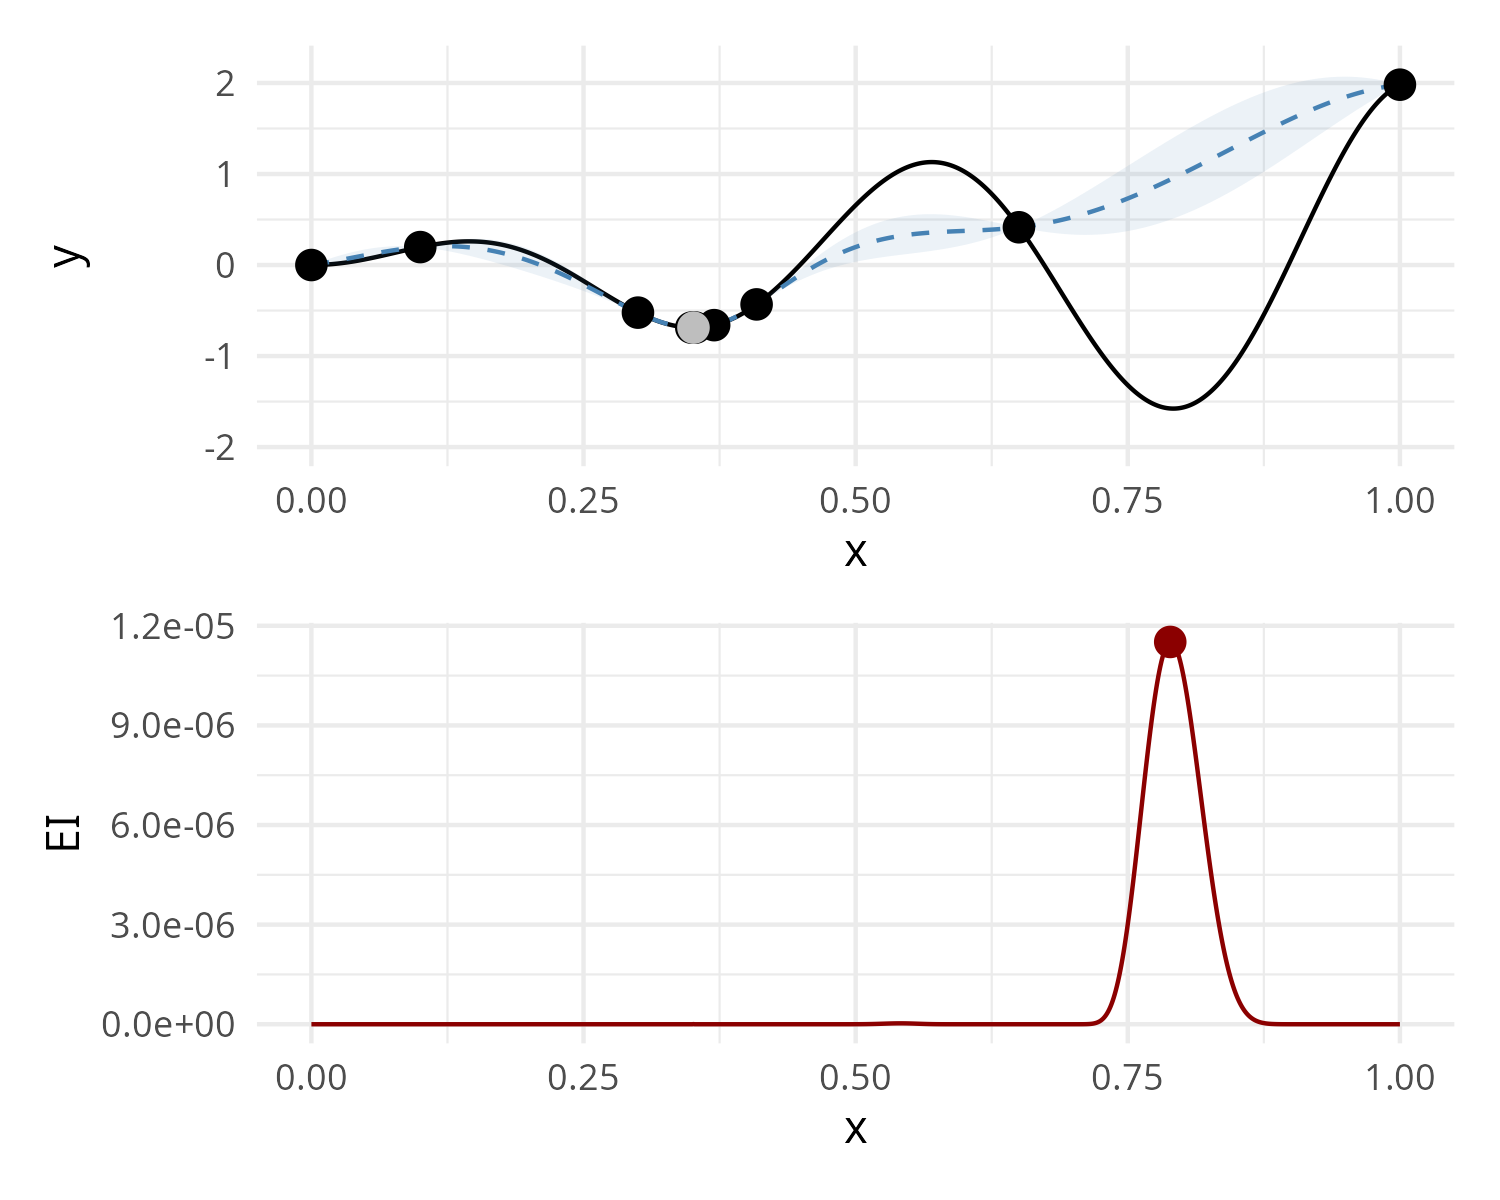
\includegraphics[width=.7\textwidth]{images/bayesian_loop_6.png}
    \end{center}
    Here, also a result of well-calibrated uncertainty $\sh(\xv)$ of our GP.
\end{frame}

%----------------------------------------------------------------------

\begin{frame}{Discussion}
    \begin{itemize}
        \item Under some mild conditions: BO with a GP as SM and EI is a \textbf{global optimizer}, i.e.\ convergence to the \textbf{global} optimum is guaranteed given unlimited budget~\liturl{Bull 2011}{https://www.jmlr.org/papers/volume12/bull11a/bull11a.pdf}
        \item Cannot be proven for the PI or the vanilla LCB
        \item LCB can be proven to converge in a similar manner if the mean-variance trade-off parameter is chosen adaptively and ``correctly''~\liturl{Srinivas et al. 2010}{https://icml.cc/Conferences/2010/papers/422.pdf}
        \item In practice, both LCB and EI work quite well
    \end{itemize}
    \vfill
    Other acquisition functions:
    \begin{itemize}
        \item Entropy-based: Entropy Search, Predictive Entropy Search, Max-value Entropy Search
        \item Knowledge Gradient
        \item Thompson Sampling
        \item \ldots
    \end{itemize}
\end{frame}

%----------------------------------------------------------------------

\begin{frame}{Summary}
\begin{enumerate}
    \item PI proposes points with highest probability of beating $\fmin$ but ignores improvement size
    \item EI maximizes expected improvement, balances exploration and exploitation, and has a closed form for Gaussian posteriors
    \item BO with GP + EI enjoys global convergence guarantees; LCB converges if $\tau$ is chosen adaptively
\end{enumerate}
\end{frame}

\end{document}
